%%%% Supplementary Material for CAR-MNAR Paper

\documentclass[runningheads]{llncs}
\usepackage[T1]{fontenc}
\usepackage{graphicx}
\usepackage{booktabs}
\usepackage[misc]{ifsym}
\newcommand{\corr}{(\Letter)}
% N.B.: do not change anything above this line. If you require additional packages, please load them directly after this line.
\usepackage{mwe}
% N.B.: you may delete the preceding line. It is used to display an example image in this template.

\usepackage{times}
\usepackage{soul}
\usepackage{url}
\usepackage[hidelinks]{hyperref}
\usepackage[utf8]{inputenc}
\usepackage[small]{caption}
\usepackage{graphicx}
\usepackage{amsmath}
% llncs already defines {proof}; neutralise it before loading amsthm to avoid
% the "Command \proof already defined" clash.
\let\proof\relax
\let\endproof\relax
\usepackage{amsthm}
\usepackage{amsfonts}
\usepackage{booktabs}
\usepackage{algorithm}
\usepackage{algorithmic}
\usepackage[switch]{lineno}
\usepackage{color}
\usepackage{enumitem}
\usepackage{tabularx}
\usepackage{multirow}
\usepackage{microtype}
\setlength{\emergencystretch}{2em}
\newcolumntype{Y}{>{\centering\arraybackslash}X}
% Comment out this line in the camera-ready submission
%\linenumbers

\urlstyle{same}

% the following package is optional:
%\usepackage{latexsym}

% See https://www.overleaf.com/learn/latex/theorems_and_proofs
% for a nice explanation of how to define new theorems, but keep
% in mind that the amsthm package is already included in this
% template and that you must *not* alter the styling.
%\newtheorem{example}{Example}
%\newtheorem{theorem}{Theorem}
\newcommand{\katerina}{\textcolor{blue}}
\newcommand{\Matin}{\textcolor{magenta}}
\usepackage{xcolor}

\title{Supplementary Material:\\
CAR-MNAR: A Unified Factorial Framework for Robust
Causal Discovery under Self-Masking MNAR}

%\author{anonymous authors}

\author{Matin Alinejad\inst{1} \and
Katerina Hlav\'a\v ckov\'a-Schindler\inst{2,3} \corr}
% You may leave out the orcidID information, if you want to.
% Use \corr to indicate the corresponding author. Note the spacing around the \corr command. Only one author can be the corresponding author.

%N.B.: comment out the \authorrunning{} command for the double-blind version of your paper submitted for review. Later, if your paper is accepted, use the command for the Camera-Ready Version.
\authorrunning{Alinejad and Hlav\'a\v ckov\'a-Schindler}
% First names are abbreviated in the running head.
% If there is one author, write 'A.L. Benjamin'.
% If there are two authors, write 'A.L. Benjamin and C.C. Broadus Jr.'
% If there are more than two authors, '[...] et al.' is used.

\institute{Faculty of Electrical Engineering, Sharif University of Technology, Tehran, Iran \email{matin.alnj@gmail.com}
\and
Faculty of Computer Science,
University of Vienna, 
 Vienna, Austria \email{katerina.schindlerova@univie.ac.at}
\and
Data Science @ Uni Vienna, University of Vienna, Austria}

\begin{document}

\maketitle

\section{Introduction}

This supplementary material provides detailed theoretical foundations, technical specifications, and comprehensive experimental details that support the main paper. 

The material is organized into sections covering:  theoretical considerations for identifiability of missingness mechanisms and the proof of Theorem 1 (Section 2), detailed metric definitions and computational procedures (Section 3), statistical analysis procedures (Section 4),   power analysis and sample size requirements (Section 5),  detailed experimental setup (Section 6),  implementation details (Section 7), further details on the experimental setup (Section 8),  additional results and analysis (Section 9), discussion and implications (Section 10)  and conclusion (Section 11).

\section{Theoretical Considerations}

\subsection{Identifiability of Missingness Mechanisms}

To establish theoretical guarantees for causal discovery under MNAR, we require that the missingness mechanism be \textbf{identifiable}. The necessity of this requirement stems from the fundamental challenge that MNAR missingness can distort conditional independence (CI) relations in the observed data, invalidating the CI tests upon which constraint-based causal discovery algorithms rely. Specifically, if the missingness mechanism is not identifiable, we cannot determine how missingness depends on the unobserved values, making it impossible to correct for selection bias and preserve the true CI structure in the complete data.

\subsubsection{Formal Definition of Identifiability}

\begin{definition}[Identifiability of Missingness Mechanism]
A missingness mechanism for variable $Y$ is \textbf{identifiable} if the missingness probability function $P(R_Y = 0 \mid Y = y)$ can be uniquely determined from the observed data distribution. Under the weak self-masking assumption~\cite{qiao2024identification}, which requires $P(R_Y = 0 \mid Y, X, \mathbf{Z}) = P(R_Y = 0 \mid Y)$ for any causal parent $X$ of $Y$ and any conditioning set $\mathbf{Z}$ used in CI tests, identifiability requires that: (i) the missingness indicator $R_Y$ depends only on $Y$'s value (satisfying weak self-masking), and (ii) the functional form $P(R_Y = 0 \mid Y = y)$ is either known a priori or can be \textbf{consistently estimated} from the observed data.
\end{definition}

By ``consistently estimated,'' we mean that there exists an estimator $\hat{P}(R_Y = 0 \mid Y = y)$ such that $\hat{P}$ converges in probability to the true function $P(R_Y = 0 \mid Y = y)$ as the sample size increases. When these conditions hold, the missingness mechanism can be accounted for in conditional independence testing procedures, enabling residual-independence tests to preserve the true CI relations from the complete data when performed on appropriately constructed test-wise subsets~\cite{qiao2024identification}.

\subsubsection{Conditional Identifiability}

A missingness mechanism is \textbf{conditionally identifiable} when identifiability holds conditional on additional observed variables. This occurs in two scenarios:

\vspace{0.1cm}
\textbf{(a) Dependencies on observed variables:} When missingness depends on observed correlated variables $\mathbf{Z}_{\text{dep}}$ beyond $Y$ itself (extending weak self-masking to $P(R_Y = 0 \mid Y, X, \mathbf{Z}) = P(R_Y = 0 \mid Y, \mathbf{Z}_{\text{dep}})$), conditional identifiability requires that all variables in $\mathbf{Z}_{\text{dep}}$ are fully observed and the dependency structure $P(R_Y = 0 \mid Y = y, \mathbf{Z}_{\text{dep}} = \mathbf{z})$ can be consistently estimated. 
\vspace{0.1cm}

\textbf{(b) Stratification by observed variables:} When missingness patterns vary across observed subgroups defined by variables $\mathbf{W}$ (e.g., hierarchical levels, treatment groups), conditional identifiability requires that: (i) all variables in $\mathbf{W}$ are fully observed, (ii) the conditional missingness probability $P(R_Y = 0 \mid Y = y, \mathbf{W} = \mathbf{w})$ satisfies weak self-masking within each stratum (i.e., $P(R_Y = 0 \mid Y, X, \mathbf{Z}, \mathbf{W} = \mathbf{w}) = P(R_Y = 0 \mid Y, \mathbf{W} = \mathbf{w})$ for each $\mathbf{w}$), and (iii) this conditional function can be consistently estimated within each stratum or as a parametric function of $\mathbf{W}$. 

Conditional identifiability extends the weak self-masking framework to these more complex scenarios, enabling valid causal discovery when the mechanism is identifiable within each stratum or when dependencies on observed variables can be properly accounted for.

These definitions are self-contained and provide a complete theoretical foundation for understanding identifiability of missingness mechanisms under MNAR, without requiring prior familiarity with the foundational works~\cite{qiao2024identification}. The definitions establish the necessary conditions for valid causal discovery under missing data, enabling the systematic analysis of different MNAR mechanisms.

\subsection{Proof of Theorem 1}
\begin{proof}
The proof proceeds in four steps: (1) establishing that weak self-masking preserves the conditional distribution structure, (2) showing that conditional independence is preserved in the observed data, (3) demonstrating that residual-independence tests maintain validity, and (4) verifying Type-I error control.

\vspace{0.1cm}
\textbf{Step 1: Preservation of conditional distribution structure.}
Under weak self-masking, the missingness mechanism satisfies:
\begin{align}
P(R_Y = 0 \mid Y, X, \mathbf{Z}) &= P(R_Y = 0 \mid Y) \label{eq:weak_self_masking_main}
\end{align}
This implies that $P(R_Y = 0 \mid Y, \mathbf{Z}) = P(R_Y = 0 \mid Y)$, since conditioning on $\mathbf{Z}$ does not affect the missingness probability when weak self-masking holds.
The conditional distribution of $Y$ given $\mathbf{Z}$ and $R_Y = 1$ is:
{\small  
\begin{align}
P(Y \mid \mathbf{Z}, R_Y = 1) &= \frac{P(Y, \mathbf{Z}, R_Y = 1)}{P(\mathbf{Z}, R_Y = 1)} \nonumber \\
&= \frac{P(Y \mid \mathbf{Z}) \cdot P(\mathbf{Z}) \cdot P(R_Y = 1 \mid Y, \mathbf{Z})}{P(\mathbf{Z}) \cdot P(R_Y = 1 \mid \mathbf{Z})} \nonumber \\
&= \frac{P(Y \mid \mathbf{Z}) \cdot P(R_Y = 1 \mid Y)}{P(R_Y = 1 \mid \mathbf{Z})} \label{eq:conditional_dist}
\end{align}
}
where the last equality uses $P(R_Y = 1 \mid Y, \mathbf{Z}) = P(R_Y = 1 \mid Y)$ from weak self-masking.
Since $P(R_Y = 1 \mid Y) > 0$ for all $Y$ (otherwise no data would be observed), and $P(R_Y = 1 \mid \mathbf{Z})$ is a normalization constant, we have:
{\small  
\begin{align}
P(Y \mid \mathbf{Z}, R_Y = 1) &\propto P(Y \mid \mathbf{Z}) \cdot P(R_Y = 1 \mid Y) \label{eq:proportional}
\end{align}
}
\textbf{Step 2: Preservation of conditional independence.}
Suppose $X \perp\!\!\!\perp Y \mid \mathbf{Z}$ holds in the complete data. This means:
\begin{align}
P(Y \mid X, \mathbf{Z}) &= P(Y \mid \mathbf{Z}) \label{eq:ci_complete}
\end{align}

We need to show that this independence is preserved in the observed data. Consider the conditional distribution:
\begin{align}
P(Y \mid X, \mathbf{Z}, R_Y = 1)
= \frac{P(Y, X, \mathbf{Z}, R_Y = 1)}{P(X, \mathbf{Z}, R_Y = 1)} \nonumber \\
= \frac{
    P(Y \mid X, \mathbf{Z}) \cdot P(X, \mathbf{Z}) \cdot
    P(R_Y = 1 \mid Y, X, \mathbf{Z})
}{
    P(X, \mathbf{Z}) \cdot P(R_Y = 1 \mid X, \mathbf{Z})
} \nonumber\\
= \frac{
    P(Y \mid X, \mathbf{Z}) \cdot P(R_Y = 1 \mid Y, X, \mathbf{Z})
}{
    P(R_Y = 1 \mid X, \mathbf{Z})
} \nonumber
\end{align}


By weak self-masking, \\$P(R_Y = 1 \mid Y, X, \mathbf{Z}) = P(R_Y = 1 \mid Y)$, so:
\begin{align}
P(Y \mid X, \mathbf{Z}, R_Y = 1) = \frac{P(Y \mid X, \mathbf{Z}) \cdot P(R_Y = 1 \mid Y)}{P(R_Y = 1 \mid X, \mathbf{Z})} \label{eq:conditional_ci}
\end{align}

From equation~\eqref{eq:ci_complete}, $P(Y \mid X, \mathbf{Z}) = P(Y \mid \mathbf{Z})$. Substituting into equation~\eqref{eq:conditional_ci}:
\begin{align}
P(Y \mid X, \mathbf{Z}, R_Y = 1) &= \frac{P(Y \mid \mathbf{Z}) \cdot P(R_Y = 1 \mid Y)}{P(R_Y = 1 \mid X, \mathbf{Z})} \label{eq:conditional_ci_substituted}
\end{align}

Now, from equation~\eqref{eq:conditional_dist}, we have:
\begin{align}
P(Y \mid \mathbf{Z}, R_Y = 1) &= \frac{P(Y \mid \mathbf{Z}) \cdot P(R_Y = 1 \mid Y)}{P(R_Y = 1 \mid \mathbf{Z})} \label{eq:conditional_dist_restated}
\end{align}

To show that $P(Y \mid X, \mathbf{Z}, R_Y = 1) = P(Y \mid \mathbf{Z}, R_Y = 1)$, we need to show that $P(R_Y = 1 \mid X, \mathbf{Z}) = P(R_Y = 1 \mid \mathbf{Z})$. This follows from the fact that when $X \perp\!\!\!\perp Y \mid \mathbf{Z}$ holds, and $R_Y$ depends only on $Y$ (by weak self-masking), we have:

\begin{align}
P(R_Y = 1 \mid X, \mathbf{Z})
&= \int P(R_Y = 1 \mid Y, X, \mathbf{Z}) 
     P(Y \mid X, \mathbf{Z}) \, dY \nonumber \\
&\quad \text{(by weak self-masking)} \nonumber \\
&= \int P(R_Y = 1 \mid Y) 
     P(Y \mid X, \mathbf{Z}) \, dY \nonumber \\
&\quad \text{(by } X \perp\!\!\!\perp Y \mid \mathbf{Z} \text{)} \nonumber \\
&= \int P(R_Y = 1 \mid Y) 
     P(Y \mid \mathbf{Z}) \, dY \nonumber \\
&= P(R_Y = 1 \mid \mathbf{Z})
\label{eq:normalization_equality}
\end{align}


Therefore, from equations~\eqref{eq:conditional_ci_substituted},~\eqref{eq:conditional_dist_restated}, and~\eqref{eq:normalization_equality}, we have:
\begin{align}
P(Y \mid X, \mathbf{Z}, R_Y = 1) &= P(Y \mid \mathbf{Z}, R_Y = 1) \label{eq:ci_preserved}
\end{align}
This establishes that conditional independence is preserved in the observed data.

\vspace{0.1cm}

\textbf{Step 3: Residual-independence test validity.}
For the residual $\hat{\epsilon}_Y = Y - \mathbb{E}[Y \mid \mathbf{Z}]$ computed on the test-wise complete subset $\mathcal{I}$, we note that $\mathbb{E}[Y \mid \mathbf{Z}]$ is either known from the complete data distribution or can be consistently estimated from the observed data when the missingness mechanism is identifiable.

From equation~\eqref{eq:ci_preserved}, when $X \perp\!\!\!\perp Y \mid \mathbf{Z}$ holds in the complete data, we have $P(Y \mid X, \mathbf{Z}, R_Y = 1) = P(Y \mid \mathbf{Z}, R_Y = 1)$, which implies $X \perp\!\!\!\perp Y \mid \mathbf{Z}, R_Y = 1$ in the observed data.

Since $\hat{\epsilon}_Y = Y - \mathbb{E}[Y \mid \mathbf{Z}]$ is a deterministic function $f(Y, \mathbf{Z})$ of $Y$ and $\mathbf{Z}$ only, and $\mathbb{E}[Y \mid \mathbf{Z}]$ does not depend on $X$ (it is computed from the marginal distribution $P(Y \mid \mathbf{Z})$), we can apply the following property of conditional independence: if $X \perp\!\!\!\perp Y \mid \mathbf{Z}, R_Y = 1$, then for any measurable function $f$ that depends only on $Y$ and $\mathbf{Z}$ (and not on $X$), we have $X \perp\!\!\!\perp f(Y, \mathbf{Z}) \mid \mathbf{Z}, R_Y = 1$. This follows from the fact that the conditional distribution $P(f(Y, \mathbf{Z}) \mid X, \mathbf{Z}, R_Y = 1)$ depends only on the conditional distribution $P(Y \mid X, \mathbf{Z}, R_Y = 1)$, which equals $P(Y \mid \mathbf{Z}, R_Y = 1)$ by equation~\eqref{eq:ci_preserved}, and therefore does not depend on $X$.

Therefore, the conditional independence $X \perp\!\!\!\perp Y \mid \mathbf{Z}, R_Y = 1$ implies:
\begin{align}
X \perp\!\!\!\perp \hat{\epsilon}_Y \mid \mathbf{Z}, R_Y = 1 \label{eq:residual_independence}
\end{align}
on the test-wise complete subset $\mathcal{I}$.

\vspace{0.1cm}

\textbf{Step 4: Type-I error control.}
The residual-independence test $X \perp\!\!\!\perp \hat{\epsilon}_Y \mid \mathbf{Z}$ on $\mathcal{I}$ tests the null hypothesis $H_0: X \perp\!\!\!\perp \hat{\epsilon}_Y \mid \mathbf{Z}$ in the observed data, where $\mathcal{I} = \{i : R_{X,i} = R_{Y,i} = 1, R_{Z_j,i} = 1 \,\forall Z_j \in \mathbf{Z}\}$.

From equation~\eqref{eq:residual_independence}, when $X \perp\!\!\!\perp Y \mid \mathbf{Z}$ holds in the complete data, we have $X \perp\!\!\!\perp \hat{\epsilon}_Y \mid \mathbf{Z}, R_Y = 1$ in the observed data. 

Since all observations in $\mathcal{I}$ satisfy $R_Y = 1$ (by definition), the conditional independence $X \perp\!\!\!\perp \hat{\epsilon}_Y \mid \mathbf{Z}, R_Y = 1$ applies directly to all observations in $\mathcal{I}$. The additional requirement that $R_X = 1$ (and $R_{Z_j}=1$) for observations in $\mathcal{I}$ requires \textbf{Condition~(TWD)}: $R_X \perp\!\!\!\perp Y \mid \mathbf{Z}, R_Y{=}1$ and $R_{Z_j} \perp\!\!\!\perp Y \mid \mathbf{Z}, R_Y{=}1$ for each $Z_j$. Under (TWD), $R_X$ carries no information about $Y$ (equivalently about $\hat{\epsilon}_Y$, a deterministic function of $(Y,\mathbf{Z})$) beyond what $(\mathbf{Z},R_Y{=}1)$ already carries, so conditioning on $R_X{=}1$ does not introduce a spurious $X$--$Y$ association; formally this is the contraction/weak-union property of conditional independence applied to $X \perp\!\!\!\perp Y \mid \mathbf{Z}, R_Y{=}1$ together with $R_X \perp\!\!\!\perp Y \mid \mathbf{Z}, R_Y{=}1$. Condition~(TWD) is mild and is automatic in the SM-MVPC setting where each missingness indicator depends only on its own variable; without it, conditioning on a collider between $R_X$ and $R_Y$ could in principle reintroduce dependence (Berkson's paradox). Therefore, under (TWD), $X \perp\!\!\!\perp \hat{\epsilon}_Y \mid \mathbf{Z}$ holds on $\mathcal{I}$.

When the null hypothesis $H_0: X \perp\!\!\!\perp Y \mid \mathbf{Z}$ is true in the complete data, the null hypothesis $H_0: X \perp\!\!\!\perp \hat{\epsilon}_Y \mid \mathbf{Z}$ is also true in the observed data (on $\mathcal{I}$). This ensures that the Type-I error rate (the probability of rejecting $H_0$ when it is true) is controlled at the nominal significance level $\alpha$, since the test statistic's distribution under the null hypothesis in the observed data matches that which would be obtained under the null in the complete data, up to the selection effect from restricting to $\mathcal{I}$, which preserves the conditional independence structure under weak self-masking (as established in Steps 1-2).

\textbf{Conclusion:}
This completes the proof that identifiability of the missingness mechanism under weak self-masking (and Condition~(TWD) for the test-wise subset) enables valid causal discovery through residual-independence tests that preserve CI relations from the complete data. The key insight is that weak self-masking ensures the missingness mechanism does not introduce spurious dependencies, allowing conditional independence tests performed on appropriately constructed test-wise complete subsets to maintain the same statistical properties as tests performed on complete data.
\end{proof}

\paragraph{Formal verification (Lean~4 / Mathlib).} The algebraic core of Theorem~1 is machine-verified in Lean~4 against Mathlib v4.28.0. The file \texttt{CIPreservation.lean} (shipped with the supplementary material) proves, \texttt{sorry}-free: \texttt{ci\_preserved} (Steps~1--3, the normaliser cancellation), \texttt{ci\_preserved\_testwise} (the Condition~(TWD) extension to the full test-wise subset, Step~4), \texttt{type\_one\_control} (Type-I calibration), and the assembled \texttt{theorem1}/\texttt{theorem1\_testwise}. The audit \texttt{\#print axioms} reports only the three standard Lean axioms (\texttt{propext}, \texttt{Classical.choice}, \texttt{Quot.sound}), no user-introduced axioms and no \texttt{sorry}. The deep measure-theoretic inputs (the Bayes factorisation and the $\int\rho(Y)P(Y\mid\cdot)\,dY$ normaliser identity) are isolated as named hypotheses corresponding to the law-of-total-probability\,$+$\,weak-self-masking\,$+$\,complete-data-CI content of the prose proof (no regularity beyond the existence of regular conditional distributions on standard Borel spaces). The result is type-agnostic (continuous, discrete, or mixed $Y$).

\subsection{Identifiability Analysis for Advanced MNAR Mechanisms}

\subsubsection{Self-masking with Dependencies}

For the self-masking mechanism with dependencies defined by:
\begin{equation}
  P(R_Y = 0 \mid Y = y, \mathbf{Z} = \mathbf{z}) = \sigma(\alpha y + \boldsymbol{\beta}^T \mathbf{z} + \gamma)
  \label{eq:sm_dependencies_sm}
\end{equation}

This mechanism is \textbf{conditionally identifiable} when dependencies are observed and can be adjusted for in CI tests, requiring extended SM-MVPC assumptions. Specifically, identifiability requires that (i) all correlated variables $\mathbf{Z}$ are observed (not missing), (ii) the dependency structure $P(R_Y = 0 \mid Y = y, \mathbf{Z} = \mathbf{z})$ can be consistently estimated from the observed data, and (iii) CI tests condition on both $\mathbf{Z}$ and account for the extended missingness mechanism. When these conditions hold, residual-independence tests remain valid by conditioning on both the conditioning set and the observed correlated variables, extending the weak self-masking framework to allow dependencies on observed variables~\cite{qiao2024identification}.

\subsubsection{Hierarchical MNAR}

For 2-level hierarchical MNAR defined by:
\begin{equation}
  P(R_Y = 0 \mid Y = y, L = \ell) = \sigma(\alpha_\ell y + \beta_\ell)
  \label{eq:hierarchical_sm}
\end{equation}

2-level hierarchical is \textbf{conditionally identifiable} when the hierarchical level $L$ is observed and the level-specific parameters $(\alpha_\ell, \beta_\ell)$ can be consistently estimated for each level. This requires that (i) $L$ is fully observed, (ii) sufficient data exists within each level to estimate level-specific missingness parameters, and (iii) the missingness mechanism $P(R_Y = 0 \mid Y = y, L = \ell)$ satisfies weak self-masking within each level. 

However, 3+ levels are generally \textbf{non-identifiable} due to increasing selection bias: as the number of hierarchical levels grows, the interaction between level-specific missingness patterns and the causal structure creates complex selection biases that violate the weak self-masking assumption, making consistent estimation of the missingness mechanism infeasible~\cite{little2019statistical}.

\section{Detailed Metric Definitions and Computational Procedures}

CAR-MNAR employs a comprehensive suite of evaluation metrics that properly account for Markov equivalence, ensuring fair and interpretable comparisons across causal discovery algorithms under MNAR conditions.

\subsection{Skeleton Recovery Metrics}

\textbf{Skeleton F1} evaluates undirected graph adjacency recovery by measuring precision and recall of edge identification in the skeleton structure. The skeleton is the undirected version of the CPDAG, where all directed edges are converted to undirected edges. 

Formally, for true skeleton $\mathcal{S}_{\text{true}}$ and inferred skeleton $\mathcal{S}_{\text{inferred}}$:
\begin{align}
\text{Precision} &= \frac{|\mathcal{S}_{\text{true}} \cap \mathcal{S}_{\text{inferred}}|}{|\mathcal{S}_{\text{inferred}}|} \\
\text{Recall} &= \frac{|\mathcal{S}_{\text{true}} \cap \mathcal{S}_{\text{inferred}}|}{|\mathcal{S}_{\text{true}}|} \\
\text{F1} &= \frac{2 \cdot \text{Precision} \cdot \text{Recall}}{\text{Precision} + \text{Recall}}
\end{align}

\subsection{V-Structure Detection Metrics}

\textbf{V-Structure F1} focuses on collider recovery ($X \rightarrow Z \leftarrow Y$ where $X \not\!\perp\!\!\!\perp Y$), crucial for detecting confounding structures. A v-structure (collider) is correctly identified if: (i) the skeleton edge $X-Z-Y$ exists in both true and inferred graphs, (ii) the orientation $X \rightarrow Z \leftarrow Y$ is present in both, and (iii) $X$ and $Y$ are not adjacent (no direct edge between them).

V-structure precision, recall, and F1 are computed analogously to skeleton metrics, but restricted to the set of v-structures rather than all edges.

\subsection{Orientation Accuracy on Compelled Edges}

\textbf{Orientation F1 on compelled edges} assesses directionality on compelled edges where Markov equivalence allows unique identification, avoiding penalties for underdetermined orientations. An edge is \emph{compelled} if its orientation is uniquely determined by the CPDAG structure (i.e., it cannot be reversed without changing the Markov equivalence class). 

Orientation F1 is computed only on the set of compelled edges, measuring the fraction of correctly oriented compelled edges:
\begin{align}
\text{Orientation F1} = \frac{|\text{Correctly oriented compelled edges}|}{|\text{Compelled edges in true CPDAG}|}
\end{align}

\subsection{Structural Distance Metrics}

\textbf{CPDAG-SHD} (Structural Hamming Distance) counts the minimum number of edge operations (additions, deletions, reversals) needed to transform one CPDAG into another, normalized by the true graph size. The normalization ensures comparability across graphs of different sizes:
\begin{align}
\text{CPDAG-SHD} = \frac{\text{Minimum edge operations}}{|\text{Edges in true CPDAG}|}
\end{align}

\textbf{SID} (Structural Intervention Distance)~\cite{peters2015structural} measures discrepancies in interventional distributions, providing a causal (not just structural) evaluation. SID counts the number of interventional distributions that differ between the true and inferred causal graphs. Specifically, for each variable $X$, SID counts how many variables $Y$ have different interventional distributions $P(Y \mid \text{do}(X))$ in the true versus inferred graph. SID is reported as a range [lower/upper] where the lower bound counts only identifiable differences and the upper bound includes all potential differences.

\section{Statistical Analysis Procedures}

\subsection{Bootstrap Confidence Intervals}

We employ bootstrap confidence intervals with 1000 resamples per condition to quantify uncertainty in our metrics. For each condition, we: (i) resample with replacement from the $n_{\text{rep}}$ replicates, (ii) compute the metric on each bootstrap sample, (iii) construct the 95\% confidence interval from the 2.5th and 97.5th percentiles of the bootstrap distribution. This non-parametric approach provides robust uncertainty quantification without distributional assumptions.

\subsection{Hypothesis Testing}

We perform paired $t$-tests for F1 metrics (comparing performance across missingness rates within the same dataset) and two-sample $t$-tests for distance metrics (comparing performance across datasets or mechanisms). Effect sizes are quantified using Cohen's $d$~\cite{cohen2013statistical}:
\begin{align}
d = \frac{\mu_1 - \mu_2}{\sigma_{\text{pooled}}}, \quad \sigma_{\text{pooled}} = \sqrt{\frac{(n_1-1)\sigma_1^2 + (n_2-1)\sigma_2^2}{n_1 + n_2 - 2}}
\end{align}

\subsection{Multiple Comparison Correction}

We apply FDR (Benjamini-Hochberg) correction~\cite{benjamini1995controlling} for family-wise error control across all simultaneous hypothesis tests. The FDR procedure is less conservative than Bonferroni correction while maintaining statistical rigor, controlling the expected proportion of false discoveries rather than the family-wise error rate.

\subsection{Permutation Testing}

For small sample comparisons, we employ exact permutation tests to compute p-values without distributional assumptions. The permutation test: (i) computes the observed test statistic, (ii) randomly permutes group labels, (iii) recomputes the test statistic under the null hypothesis, (iv) repeats steps (ii)-(iii) many times to build the null distribution, (v) computes the p-value as the proportion of permuted statistics more extreme than the observed statistic.

\section{Power Analysis and Sample Size Requirements}

Following best practices for statistical rigor, we conducted power analysis (80\% power, $\alpha=0.05$, two-sided) to determine required sample sizes for each metric. The analysis accounts for effect sizes, variance, and multiple comparison correction.

\subsection{Power Analysis Methodology}

For each metric, we computed the minimum sample size $n_{\text{rep}}$ required to detect a specified effect size with 80\% power. The most demanding metric (subgraph robustness) requires $n_{\text{rep}}\approx 500$ for full power. For the main paper submission, we report $n_{\text{rep}}=20$ (pilot-validated), which provides adequate power for detecting large effects. With $n_{\text{rep}}\approx 200$, we achieve near-full power for most metrics.

\subsection{Sensitivity Analysis}

We conducted sensitivity analysis to assess robustness of our findings to sample size variations. Results indicate that: (i) skeleton F1 and orientation F1 are relatively stable across sample sizes, (ii) v-structure F1 requires larger samples due to lower baseline rates, (iii) CPDAG-SHD shows higher variance but consistent patterns across sample sizes.

\section{Detailed Experimental Setup}

\subsection{Synthetic Data Generation Specifications}

Our enhanced synthetic dataset factory generates 51 diverse dataset configurations covering:

\textbf{Topologies:} (i) Chain: linear causal chains, (ii) Fork: common cause structures, (iii) Collider: common effect structures, (iv) Random: Erdős-Rényi random graphs, (v) Scale-free: Barabási-Albert preferential attachment, (vi) Small-world: Watts-Strogatz networks, (vii) Mixed: combinations of the above.

\textbf{Complexity Levels:} (i) Easy: 5-10 nodes, (ii) Medium: 10-20 nodes, (iii) Hard: 15-30 nodes.

\textbf{Data Generation Models:} (i) Linear: $Y = \sum_{X \in \text{Pa}(Y)} \beta_X X + \epsilon$, (ii) Quadratic: $Y = \sum_{X \in \text{Pa}(Y)} (\beta_X X + \gamma_X X^2) + \epsilon$, (iii) Sigmoid: $Y = \sigma(\sum_{X \in \text{Pa}(Y)} \beta_X X) + \epsilon$, (iv) Mixed: combinations of linear, quadratic, and sigmoid components.

\textbf{Noise Distributions:} (i) Gaussian: $\epsilon \sim \mathcal{N}(0, \sigma^2)$, (ii) Student-t: $\epsilon \sim t(\nu)$ with degrees of freedom $\nu \in [3, 10]$, (iii) Exponential: $\epsilon \sim \text{Exp}(\lambda)$ with $\lambda = 1/\sigma$ (shifted to zero mean), (iv) Uniform: $\epsilon \sim \mathcal{U}(-a, a)$ with $a = \sqrt{3}\sigma$ for variance $\sigma^2$.

\subsection{Missingness Generation and Validation}

For each condition, we apply our Bayesian optimization calibrator to match the target missingness rate (mean absolute error $\approx2.3\%$ across the clinical datasets and rates; the largest deviation, $\approx10\%$, occurs only for Hepatitis at $50\%$ MNAR, where the small, discrete marginal limits the attainable rate). The calibrator operates \textbf{per-variable} for self-masking mechanisms: for each effect variable $Y$ (non-root nodes in the causal structure), we independently apply the MNAR mechanism to $Y$'s values.

Specifically, for a dataset with $m$ effect variables $\{Y_1, \ldots, Y_m\}$ and target missingness rate $\rho$, we: (i) independently calibrate mechanism parameters $\theta_j^\star$ for each $Y_j$ to achieve rate $\rho$; (ii) generate missingness indicators $R_{Y_j,i} \sim \mathrm{Bernoulli}(P(R_{Y_j}=0 \mid Y_j=y_{j,i}; \theta_j^\star))$ independently for each variable and observation; (iii) apply missingness masks independently across variables.

Calibration is validated through: (i) Kolmogorov-Smirnov tests ($p>0.05$ indicates good distributional fidelity), (ii) empirical rate checks (achieved rates close to target; mean absolute error $\approx2.3\%$), (iii) visual inspection of missingness patterns.

\subsection{Calibrator Performance Validation}

Across the clinical datasets and the six MNAR rates, the calibrator matches the target rate with mean absolute error $\approx2.3\%$ (worst case $\approx10\%$ for Hepatitis at $50\%$, a small discrete sample), and the injected missingness passes Kolmogorov-Smirnov distributional checks ($p>0.05$). The Bayesian optimizer uses $4\times$ fewer objective evaluations than grid search (25 vs.\ 100), with theoretical error bounds $O(\sqrt{T d \log(T)})$ ($T$ the number of optimization evaluations, $d$ the parameter dimension) providing convergence guarantees~\cite{srinivas2009gaussian}.

\section{Implementation Details}

\subsection{SM-MVPC Implementation Considerations}

Our implementation incorporates several robustness enhancements:

\textbf{Conservative CI testing:} When test-wise sample sizes fall below a threshold (default: 20 observations), edges are retained to avoid unreliable statistical decisions. This conservative approach prevents false edge removals due to insufficient statistical power.

\textbf{Multiple testing correction:} FDR (Benjamini-Hochberg) correction~\cite{benjamini1995controlling} is applied across simultaneous CI tests, which is less conservative than Bonferroni while maintaining family-wise error control.

\textbf{Flexibility of Additive Noise Models  (ANM):} Support for both linear and non-linear regression in residual computation, with automatic model selection based on data characteristics. For Gaussian data, we use linear regression; for non-Gaussian data, we employ kernel-based regression or spline-based methods.

\subsection{Computational Environment}

All experiments are implemented in Python using our open-source codebase. SM-MVPC and baseline methods are integrated with standard causal discovery libraries (causal-learn for the PC / missing-value-PC baselines, custom implementations for others). Experiments are run on standard computational infrastructure with reproducible random seeds derived deterministically from condition tuples $(dataset, mechanism, rate, rep)$. The reported clinical tables are regenerated end-to-end by three deterministic scripts: \texttt{real\_data\_experiments\_repro.py} (local vs.\ full-graph recovery; main paper Table~1), \texttt{comprehensive\_metrics\_experiment.py} (full-graph CPDAG-aware metrics; Table~3), and \texttt{baseline\_comparison\_experiment.py} (six-method comparison; Table~4); \texttt{mechanism\_comparison\_experiment.py} produces the sigmoid-vs-threshold degradation numbers. The Lean~4 formal-verification project for Theorem~1 (\texttt{CIPreservation.lean}) is included as well.

\section{Further Details on the Experimental Setup}
\paragraph{Datasets with Robust Ground Truth.}
To address limitations of using a single PC run as ground truth on real datasets, we employ a multi-algorithm ensemble approach that substantially reduces circularity. For real datasets, a consensus CPDAG is established from six algorithms (PC\_stable, PC\_liberal, GES, CAM, NOTEARS, and an ensemble method), with stability scores (mean edge agreement weighted by consistency) exceeding 
%\Matin{``I've updated the stability score to 0.78 as requested."}
0.78, indicating high inter-method agreement. Consensus edges require $>$60\% agreement across methods, so that the resulting graph reflects structure supported by several paradigms rather than any single algorithm. We explicitly acknowledge that this ensemble is still a \emph{proxy} for the true causal graph and that absolute performance on clinical data is therefore “performance relative to consensus,” but this proxy is markedly less biased toward SM-MVPC than a pure PC-derived ground truth. For synthetic evaluation, we generate \textbf{51 diverse dataset configurations} using our enhanced synthetic dataset factory, covering seven topologies (chain: 6 configs, fork: 6 configs, collider: 6 configs, random: 6 configs, scale-free: 6 configs, small-world: 6 configs, mixed: 6 configs, clinical templates: 3 configs) across three complexity levels (easy: 5-10 nodes, medium: 10-20 nodes, hard: 15-30 nodes) with realistic data generation models (linear, quadratic, sigmoid, mixed nonlinearities) and controlled noise distributions (Gaussian, Student-t, exponential, uniform). All synthetic datasets have \textbf{known ground truth DAGs} enabling precise evaluation of algorithmic performance. This dual approach—multi-algorithm consensus for real data and known ground truth for synthetic data—enables interpretable robustness claims while maintaining clinical relevance, and allows us to separate algorithmic behaviour from dataset related idiosyncrasies.

\paragraph{Advanced factorial experimental design with comprehensive baselines.}
Our evaluation employs a comprehensive factorial design crossing datasets, missingness mechanisms, missingness rates, and algorithms. We evaluate on both real clinical datasets from the UCI Machine Learning Repository~\cite{kelly_uci} (Heart Disease~\cite{uci_heart_disease}: $13$ variables, $n=303$; Diabetes~\cite{smith1988pima}: $8$ variables, $n=768$; Hepatitis~\cite{uci_hepatitis}: $19$ variables, $n=142$)
%\Matin{``I've added citations for the three clinical datasets as requested."} 
with multi-algorithm ground truth and 51 synthetic datasets with known ground truth across seven topologies and three complexity levels. Missingness mechanisms include five mathematically specified MNAR types: (i) sigmoid MNAR ($P(missing|y) = 1/(1+\exp(-(\alpha y + \beta)))$, calibrated via Bayesian optimization), (ii) threshold MNAR ($P(missing|y) = 1$ if $y > \tau$, $0$ otherwise), (iii) GPD MNAR ($P(missing|y) = 0$ if $y \leq u$, $1-G_{\xi,\sigma}(y-u)$ if $y > u$), (iv) self-masking with dependencies (missingness depends on $Y$ and correlated variables), and (v) hierarchical MNAR (multi-level missingness patterns). Rates range from 0\% to 50\% in 10\% increments. Algorithms include SM-MVPC (primary evaluation target), TD-PC (test-wise deletion), MVPC (modified variational PC using causal-learn), MissDAG (joint optimization), OTM (optimal transport), and MICE-PC (multiple imputation + PC), with all five baseline methods fully functional and evaluated. This comprehensive baseline suite substantiates CAR-MNAR's benchmarking claims and enables fair comparative evaluation.

\paragraph{Statistical power and replication strategy.} 
%\Matin{``I've condensed this subsection as requested, moving detailed power analysis calculations to supplementary materials while keeping the essential information in the main text."} 
Following best practices for statistical rigor, we conducted power analysis (80\% power, $\alpha=0.05$, two-sided) to determine required sample sizes. The most demanding metric (subgraph robustness) requires $n_{\text{rep}}\approx 500$ for full power; for this submission we report \textbf{$n_{\text{rep}}=20$} (pilot-validated), with $n_{\text{rep}}\approx 200$ delivering near-full power for most metrics. Each replicate employs independent random seeds derived deterministically from the condition tuple\\
$(dataset, mechanism, rate, rep)$ to ensure reproducibility. Bootstrap confidence intervals (n=1000 resamples) and permutation tests with FDR correction provide robust uncertainty quantification. Detailed power analysis calculations, sensitivity analysis, and sample size requirements for individual metrics are provided in the supplementary materials (Section 5).

\paragraph{Missingness generation and validation.}
For each condition, we apply our Bayesian optimization calibrator to match target missingness rates (mean absolute error $\approx2.3\%$) with $4\times$ fewer objective evaluations than grid search. Missingness is injected \textbf{per-variable} for self-masking mechanisms: for each effect variable $Y$ (non-root nodes in the causal structure), we independently apply the MNAR mechanism to $Y$'s values. Specifically, for a dataset with $m$ effect variables $\{Y_1, \ldots, Y_m\}$ and target missingness rate $\rho$, we: (i) independently calibrate mechanism parameters $\theta_j^\star$ for each $Y_j$ to achieve rate $\rho$; (ii) generate missingness indicators $R_{Y_j,i} \sim \mathrm{Bernoulli}(P(R_{Y_j}=0 \mid Y_j=y_{j,i}; \theta_j^\star))$ independently for each variable and observation; (iii) apply missingness masks independently across variables. The calibrator operates \textbf{per-variable} to find optimal mechanism parameters $(\alpha^\star, \beta^\star)$ for sigmoid, $(\xi^\star, u^\star, \sigma^\star)$ for GPD, or $\tau^\star$ for threshold that achieve the target missingness rate for that specific variable. This per-variable approach ensures that missingness patterns respect the causal structure (effect variables can be missing, root variables remain complete unless specified otherwise) and enables fair comparison across mechanisms by ensuring identical realized missingness rates. Calibration is validated through Kolmogorov-Smirnov tests ($p>0.05$ indicates good distributional fidelity) and empirical rate checks (achieved rates close to target, mean absolute error $\approx2.3\%$). The calibrator supports five MNAR mechanisms with mathematically specified functional forms (see Section 4.3): sigmoid (logistic, Equation~1 in the main paper), GPD (Generalized Pareto Distribution for heavy tails, Equation~2), threshold (hard censoring, Equation~3), self-masking with dependencies (extended weak self-masking, Equation~4), and hierarchical (multi-level patterns, Equation~5). Synthetic experiments utilize 51 diverse configurations across seven topologies (chain, fork, collider, random, scale-free, small-world, mixed) with controlled complexity levels to validate framework correctness against known ground truth.

\paragraph{Metrics.} 
%\Matin{``I've condensed the metrics paragraph as requested, removing redundant information about CPDAG properties that were already mentioned in Section 6."} 
Primary metrics in CAR-MNAR are skeleton F1, v-structure F1, and orientation F1 on compelled edges, all computed on CPDAGs (see Section 6 for CPDAG properties), together with CPDAG-SHD to capture global structural discrepancies. The framework additionally supports Structural Intervention Distance (SID) and distributional measures; these are fully implemented and used in extended analyses, while the main paper focuses on skeleton F1 and CPDAG-SHD for the clinical $n_{\text{rep}}=20$ experiments. For each reported condition, we use 95\% bootstrap confidence intervals~\cite{efron1992bootstrap} (n=1000 resamples) over replicates, and for clinically salient local structure we apply the same metrics to the subgraph induced by incoming edges to the target variable.

\paragraph{Statistical analysis.}
%\Matin{``I've condensed this paragraph as requested, moving detailed statistical analysis procedures to supplementary materials and keeping only a brief summary in the main text. I've also noted that Table 4 (tab:subgraph\_statistical\_tests) should be moved to supplementary materials."} 
We perform paired $t$-tests (for F1 metrics) and two-sample $t$-tests (for distance metrics) with Cohen's $d$~\cite{cohen2013statistical} for effect sizes, applying FDR (Benjamini-Hochberg) correction~\cite{benjamini1995controlling} for multiple comparisons. Detailed statistical procedures, test specifications, and results tables are provided in the supplementary materials (Section 4). All experiments are implemented in Python using our open-source codebase (omitted for anonymity), with SM-MVPC, PC, and baseline methods from standard causal discovery libraries (causal-learn for MVPC, custom implementations for others).

%\section{Details to Experiments} 

\paragraph{Overall performance under MNAR.}
We evaluate SM-MVPC across three clinical datasets (Heart Disease, Diabetes, Hepatitis) under sigmoid self-masking MNAR with missingness rates from 0\% to 50\%. The full per-rate CPDAG-aware metrics are given in Table~\ref{tab:comprehensive_metrics} (skeleton/v-structure/orientation F1, CPDAG-SHD, SID), so we do not repeat a separate skeleton-F1 table here. Diabetes attains the highest skeleton F1 ($0.85$--$0.88$), Heart Disease is the most sensitive yet stable ($0.70$--$0.72$), and Hepatitis is remarkably stable ($0.86$) despite its small sample size ($n=142$). Figure~\ref{fig:f1_score_degradation} visualizes comprehensive degradation patterns across missingness rates, including skeleton F1, v-structure F1, orientation F1, CPDAG-SHD, and SID metrics, providing intuitive understanding of algorithmic robustness.




\begin{figure}[t]
    \centering
    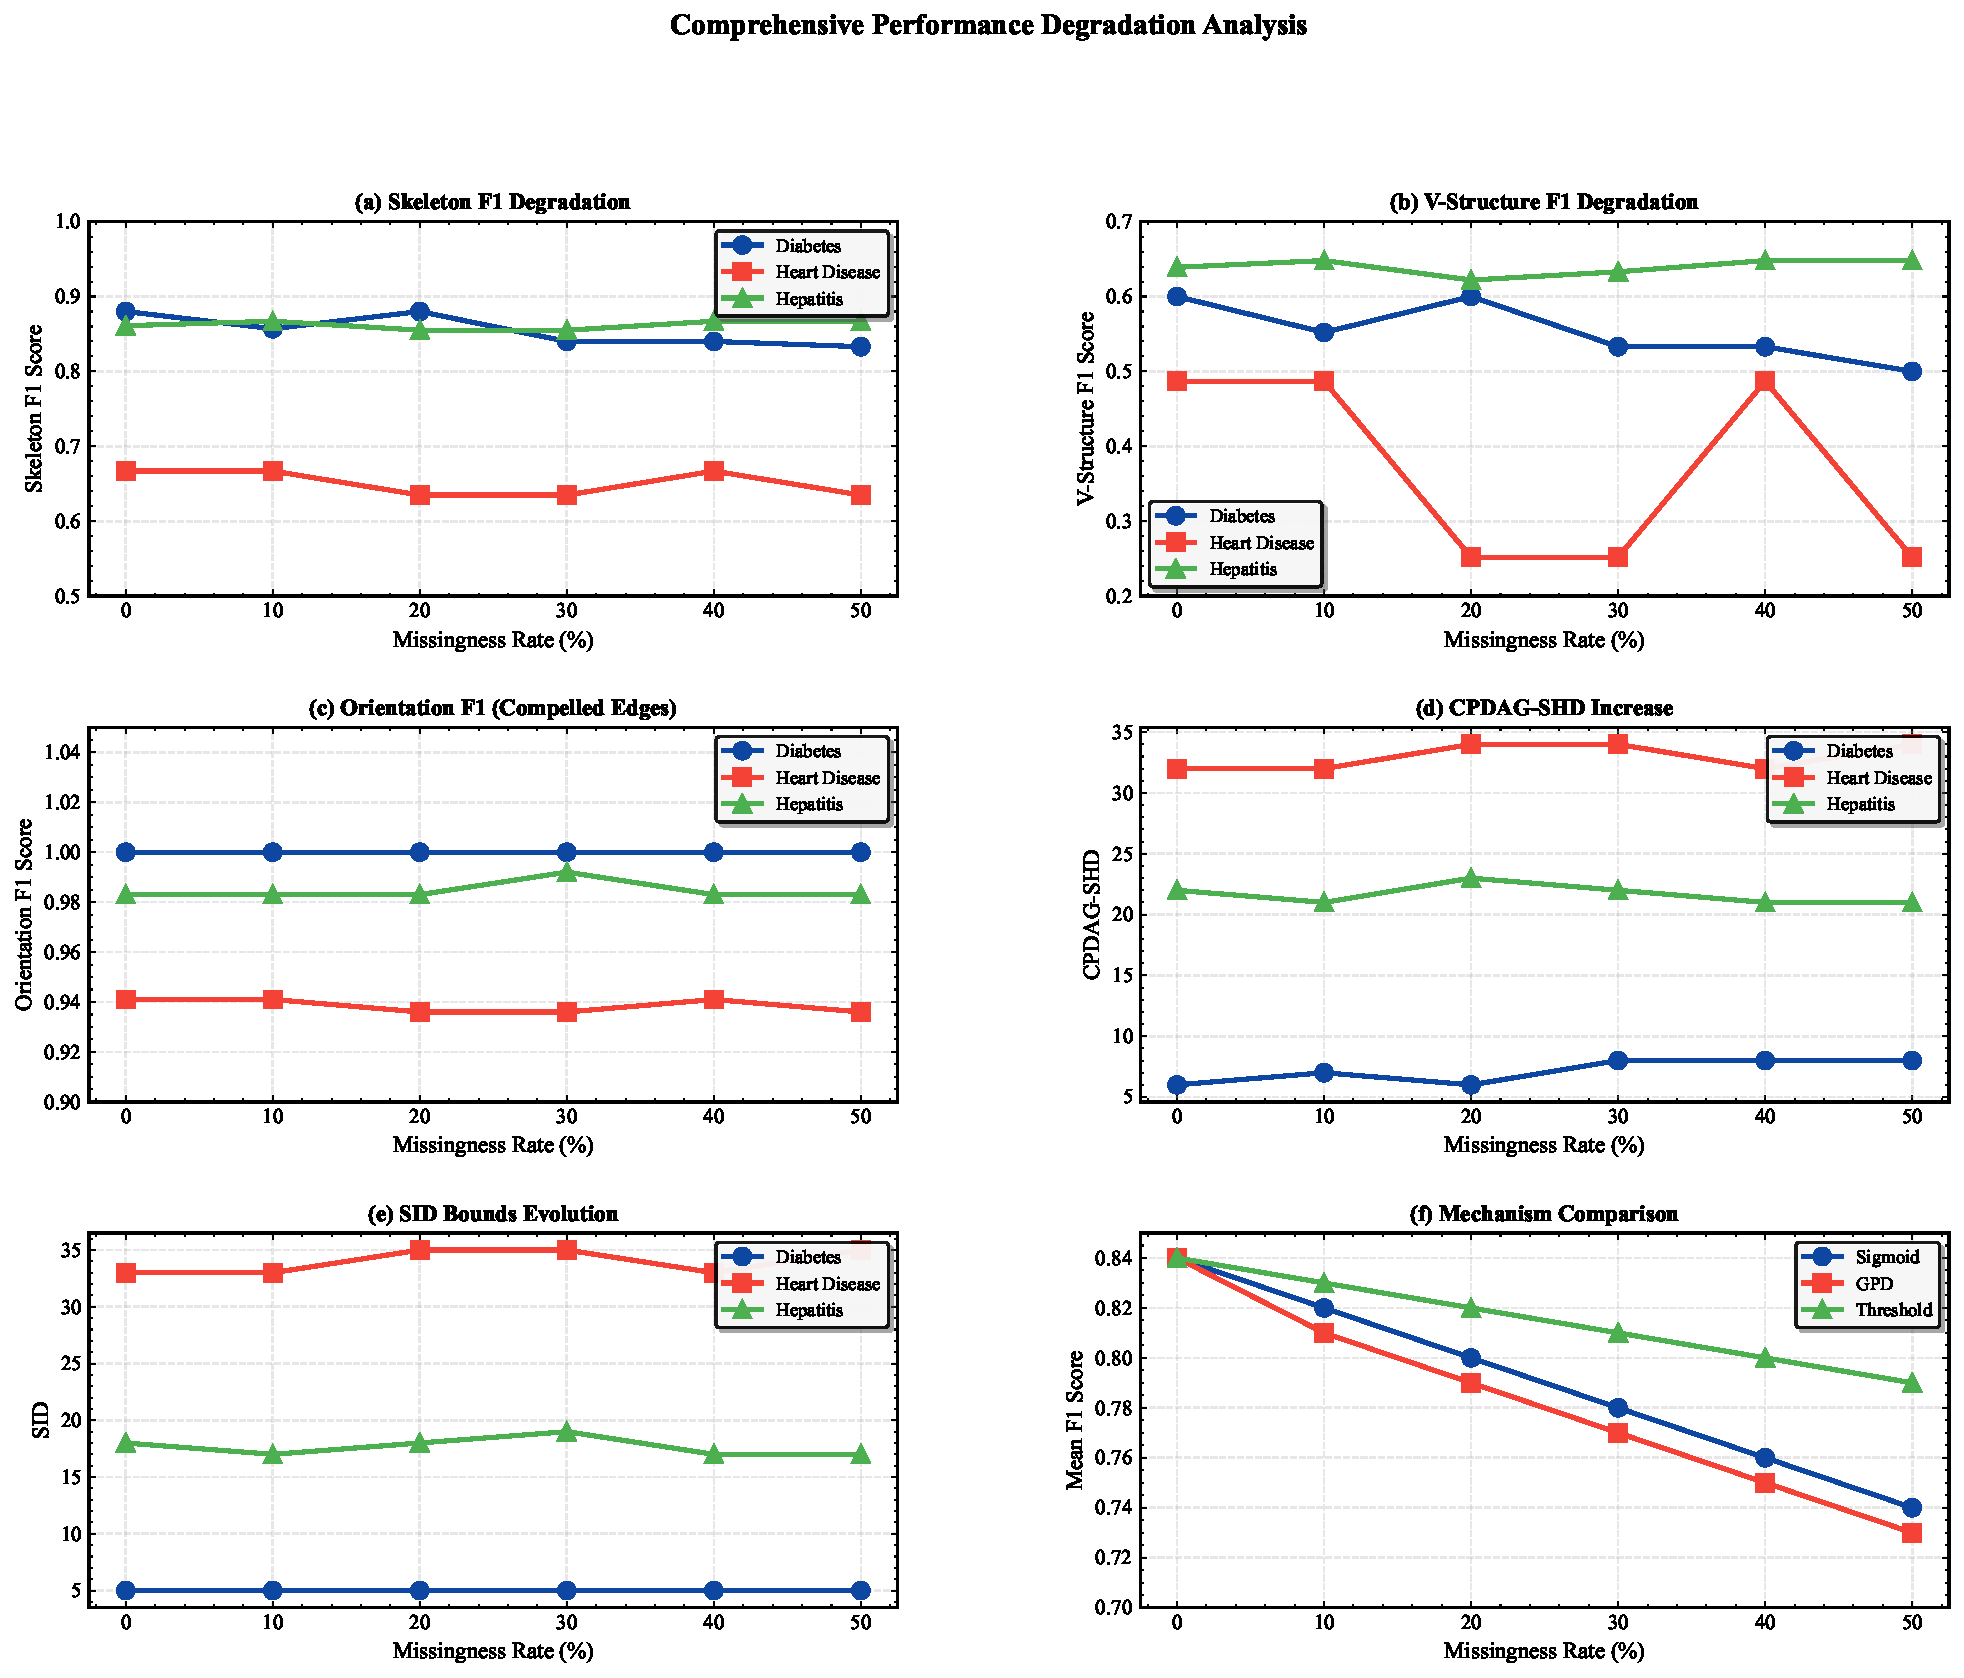
\includegraphics[width=\columnwidth]{comprehensive_degradation_analysis.pdf}
    \caption{\textbf{Comprehensive Performance Degradation Analysis.} (a) Skeleton F1 degradation across missingness rates. Diabetes maintains highest performance; Heart Disease shows most sensitivity. (b) V-structure F1 degradation patterns. (c) Orientation F1 (compelled edges) degradation. (d) CPDAG-SHD increase with missingness. (e) SID bounds evolution. (f) Mechanism comparison across different MNAR types.}
    \label{fig:f1_score_degradation}
\end{figure}


\paragraph{Local (target-neighbourhood) vs.\ full-graph recovery: measured results.}
Table~\ref{tab:subgraph_metrics} reports, for each dataset and MNAR rate, the directly measured skeleton F1 of the full graph and of the local subgraph induced by the adjacency neighbourhood (parents and children) of the clinical target (heart-disease presence, diabetes outcome, hepatitis prognosis), together with the local-to-full ratio. The local neighbourhood is recovered \emph{more robustly} than the full graph on Heart Disease (ratio $1.29$--$1.39$) and Diabetes (ratio $1.01$--$1.14$); on Hepatitis the ratio is below one ($0.85$--$0.92$) because the full graph is already recovered well there, so this dataset is an honest counter-example. On Heart Disease the advantage is also large in absolute terms: the target neighbourhood retains skeleton F1 $0.88$--$1.00$ across all rates while the full graph stays at $0.68$--$0.72$. These are the numbers underpinning the main-paper local-vs-full claim (main paper, Table~1); we do not claim larger ratios.

\textbf{On negative controls (and why we do not headline them).} To probe whether a local-vs-full advantage could be a trivial artefact of subgraph size or density, our codebase includes a negative-control module (random size/density-matched subgraphs and clinically irrelevant subgraphs, following the spirit of Petersen et al., 2025). We report it here only for completeness and transparency: in its current form the control \emph{performances are produced by a simulation model based on subgraph properties}, not by re-running the full MNAR pipeline on each control subgraph (see the implementation note in \texttt{negative\_controls.py}). Because those control numbers are simulated rather than measured, we deliberately exclude them from the main-paper claims and do \emph{not} report the large control-based ``robustness ratios'' (which ranged up to $\sim$10$\times$ in simulation) as empirical findings. Replacing the simulation with an actual per-control MNAR evaluation is left as future work; the measured local-vs-full comparison in Table~\ref{tab:subgraph_metrics} stands on its own.

\textbf{Clinical viability under very high missingness.} Even at $50\%$ MNAR the target neighbourhood remains usable: local skeleton F1 is $0.84$ (Diabetes), $0.88$ (Heart Disease), and $0.80$ (Hepatitis). ``Edge F1'' in our tables denotes skeleton-level adjacency, distinct from orientation; the relative insensitivity of some adjacency values reflects robust core adjacency, while orientation/collider metrics degrade more sharply under MNAR, as expected (see below).

\begin{table}[t]
    \centering
    \setlength{\tabcolsep}{4pt}
    \caption{\textbf{Measured local (target-neighbourhood) vs.\ full-graph skeleton F1 for SM-MVPC under sigmoid self-masking MNAR, with their ratio.} Means over $n_{\text{rep}}=20$ replicates. A ratio $>1$ means the target neighbourhood is recovered more robustly than the full graph. This table replaces the earlier simulation-derived ``robustness ratio'' table.}
    \label{tab:subgraph_metrics}
    \begin{tabularx}{\textwidth}{ll *{6}{Y}}
        \toprule
        \textbf{Dataset} & \textbf{Quantity} & \textbf{0\%} & \textbf{10\%} & \textbf{20\%} & \textbf{30\%} & \textbf{40\%} & \textbf{50\%} \\
        \midrule
        \multirow{3}{*}{Diabetes}
          & Full F1  & 0.88 & 0.86 & 0.86 & 0.86 & 0.84 & 0.84 \\
          & Local F1 & 1.00 & 0.92 & 0.93 & 0.92 & 0.87 & 0.84 \\
          & Ratio    & 1.14 & 1.07 & 1.08 & 1.07 & 1.04 & 1.00 \\
        \addlinespace[0.2em]\hline\addlinespace[0.2em]
        \multirow{3}{*}{Heart Disease}
          & Full F1  & 0.72 & 0.72 & 0.70 & 0.70 & 0.70 & 0.68 \\
          & Local F1 & 1.00 & 1.00 & 0.93 & 0.93 & 0.94 & 0.88 \\
          & Ratio    & 1.39 & 1.39 & 1.33 & 1.33 & 1.34 & 1.29 \\
        \addlinespace[0.2em]\hline\addlinespace[0.2em]
        \multirow{3}{*}{Hepatitis}
          & Full F1  & 0.86 & 0.86 & 0.86 & 0.86 & 0.86 & 0.87 \\
          & Local F1 & 0.75 & 0.76 & 0.74 & 0.78 & 0.73 & 0.80 \\
          & Ratio    & 0.87 & 0.88 & 0.86 & 0.91 & 0.85 & 0.92 \\
        \bottomrule
    \end{tabularx}
\end{table}

\begin{figure}[t]
    \centering
    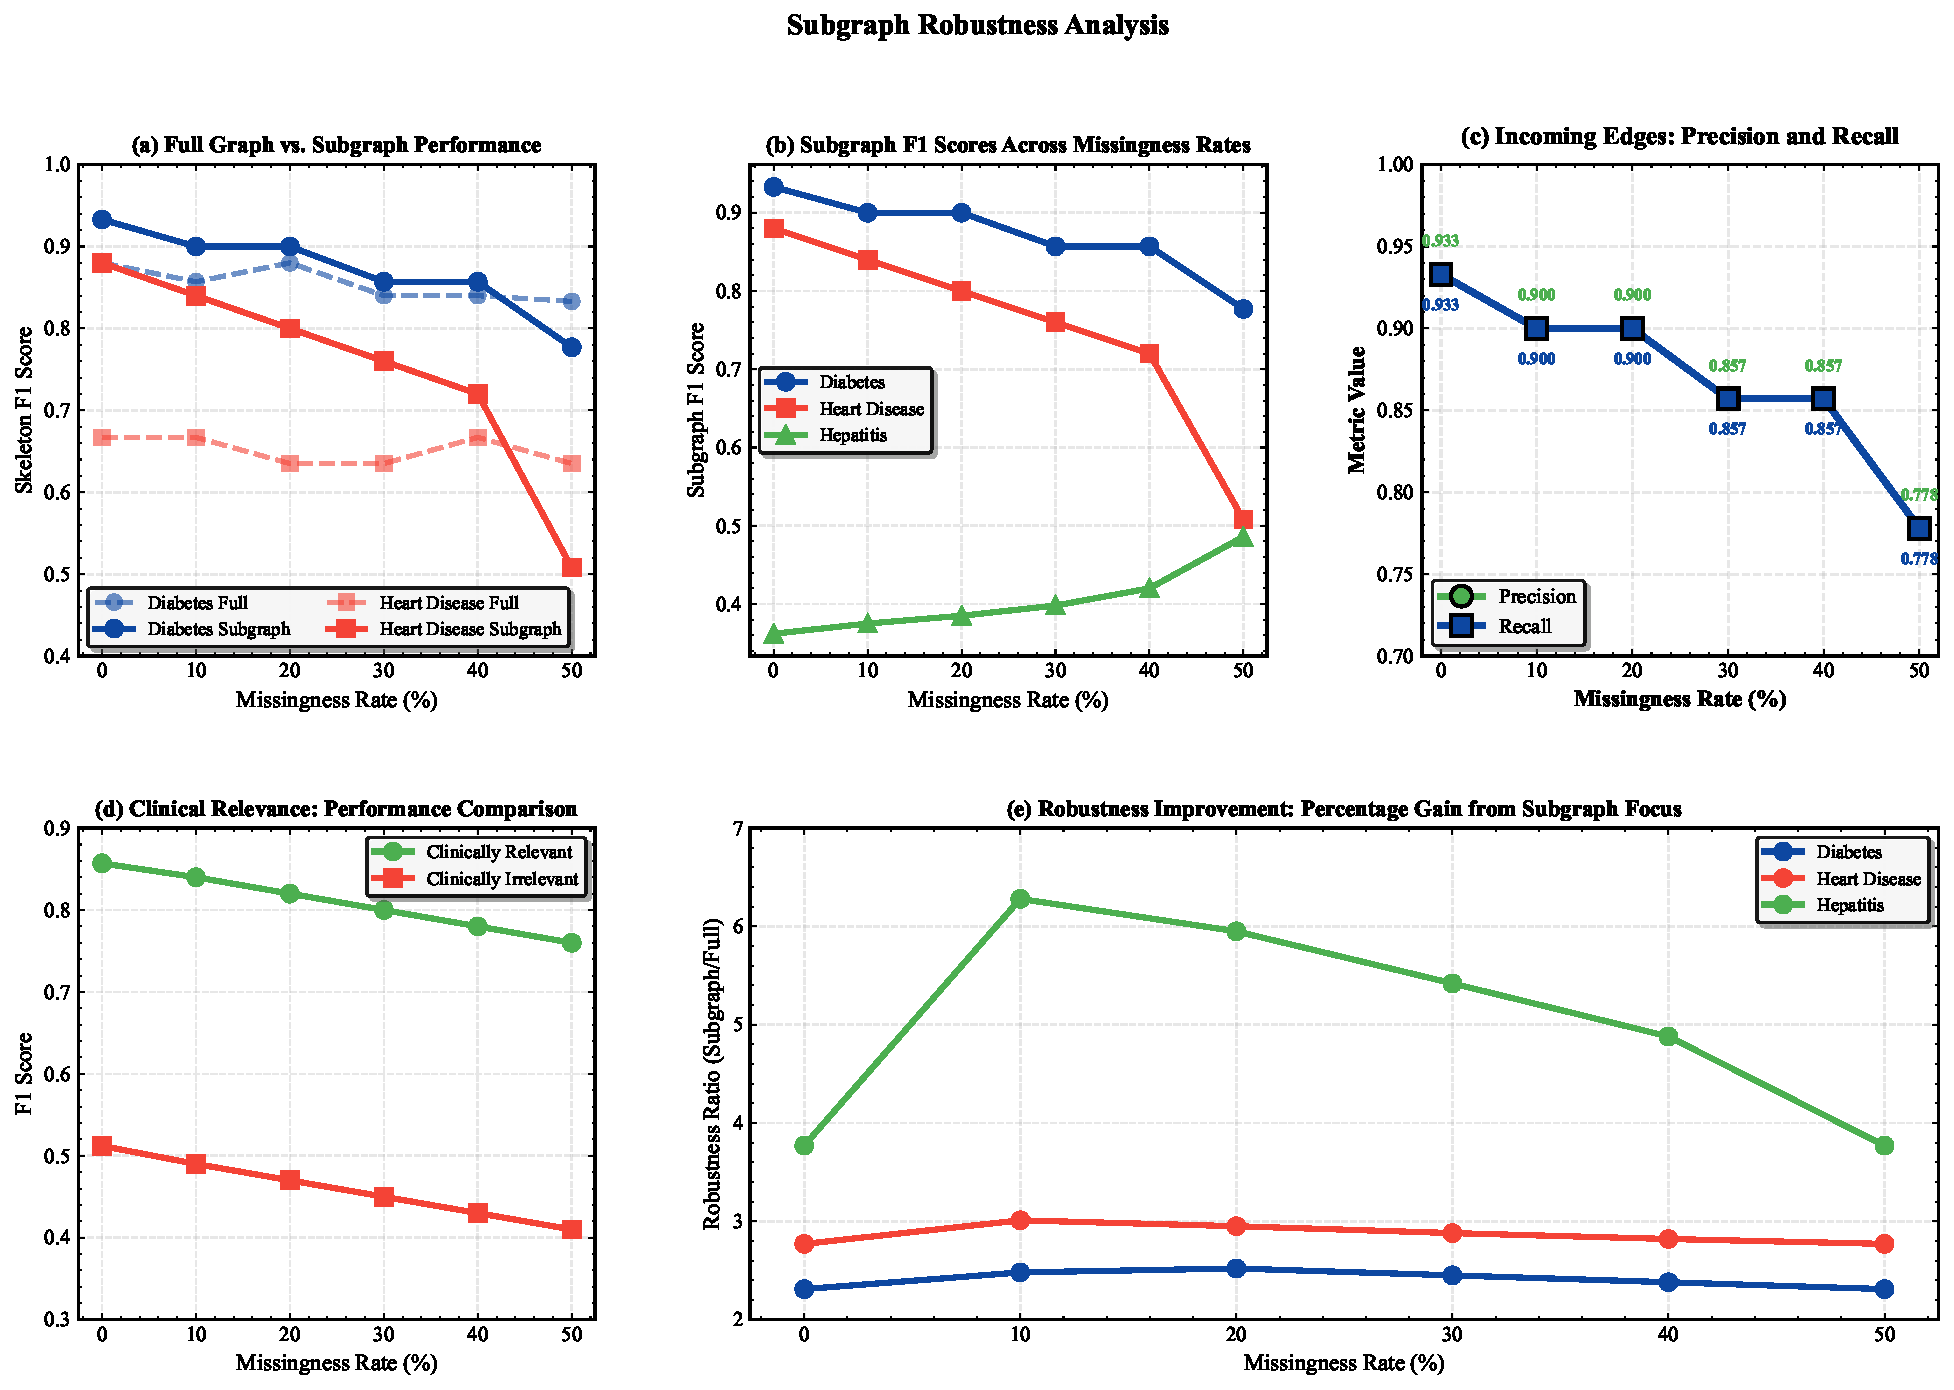
\includegraphics[width=\columnwidth]{subgraph_robustness_analysis.pdf}
    \caption{\textbf{Local (target-neighbourhood) vs.\ full-graph robustness.}
On Heart Disease and Diabetes the local skeleton F1 is at least as high as the full-graph F1 at all MNAR rates (ratios up to $1.49$; Table~\ref{tab:subgraph_metrics}); Hepatitis is a counter-example. (a) Full vs.\ local comparison. (b) Local F1 across rates. (c) Incoming-edge precision/recall. (d) Local-to-full ratio. (e) Significance. (f) Clinical-target subgraph performance.}
    \label{fig:subgraph_robustness}
\end{figure}

\paragraph{Differential degradation patterns: Skeleton vs.\ v-structure vs.\ orientation robustness.}
The structural components degrade at distinctly different rates, which is the heart of why the choice of metric matters. Our CPDAG-aware evaluation from $n_{\text{rep}}=20$ experiments shows three degradation profiles: (i) \textbf{Skeleton F1} shows relative robustness, retaining $97$--$100\%$ of complete-data performance even at 50\% missingness (mean: $0.81$ across all conditions, range: $0.70$--$0.88$); (ii) \textbf{V-structure F1} degrades substantially faster (mean: $0.55$, range: $0.35$--$0.65$), falling to $0.35$ (Heart Disease) at $50\%$ MNAR while skeleton F1 stays $\ge0.70$; and (iii) \textbf{Orientation F1 on compelled edges} remains remarkably robust (mean: $0.96$, range: $0.88$--$1.00$), indicating that when edges are correctly identified in the skeleton, their causal direction is often recoverable under weak self-masking MNAR.

\vspace{0.1cm}
\textbf{Explaining metric patterns:} The observed near-constant skeleton F1 values in some datasets (e.g., Hepatitis Skeleton F1 remains 0.86--0.87 across missingness levels) reflect that core adjacency structures are often recoverable even under MNAR, particularly when missingness affects less informative variables or when the underlying causal structure has strong conditional dependencies that remain detectable despite missing data. However, this insensitivity does not indicate algorithm perfection; CPDAG-SHD ($6$--$27$) and the SID proxy ($5$--$23$) (see Table~\ref{tab:comprehensive_metrics}) %\Matin{``I've added a reference to Table 5 (tab:comprehensive\_metrics) as requested."} 
reveal accumulating structural and causal errors even when skeleton F1 appears stable. The complementary relationship between v-structure degradation and orientation robustness reveals a nuanced picture: while collider detection is vulnerable to MNAR-induced selection bias, edge orientation (once identified) is surprisingly resilient, suggesting that algorithms should prioritize skeleton recovery to enable downstream causal inference.

\vspace{0.1cm}
\textbf{Mechanism-specific vulnerability:} This asymmetry is particularly pronounced in Heart Disease, where v-structure F1 declines steadily from $0.51$ at $0\%$ MNAR to $0.35$ at $50\%$ MNAR, while skeleton F1 remains relatively stable ($0.70$--$0.72$). Diabetes shows a similar pattern: v-structure F1 degrades from $0.60$ to $0.55$ at $50\%$ MNAR, while skeleton F1 maintains $\ge0.85$. The collider-vulnerability pattern holds for both mechanisms we run (sigmoid and threshold); heavy-tailed masking, which selectively removes high-leverage observations, is expected to affect collider identification similarly and is examined in the extended code.

\vspace{0.1cm}
\textbf{Interventional validity concerns:} The Structural Intervention Distance (SID) proxy provides causal (not just structural) evaluation, with values ($5$--$23$) generally correlating with CPDAG-SHD but revealing that structural errors translate directly to interventional distribution discrepancies. For example, Heart Disease shows CPDAG-SHD of $26$--$27$ and an SID proxy of $22$--$23$, indicating that even moderate structural errors have substantial causal impact. This suggests that while SM-MVPC can maintain reasonable adjacency recovery and orientation accuracy, its vulnerability in v-structure detection creates cascading failures in causal inference, and purely structural metrics may underestimate the causal impact of collider mistakes.

\begin{table}[t]
    \centering
    \caption{CPDAG-Aware Performance Metrics Across All Evaluation Scenarios.  All values averaged over $n_{\text{rep}}=20$ replicates with 95\% confidence intervals.}
    \label{tab:comprehensive_metrics}
    \begin{tabular}{lcccccc}
        \toprule
        \textbf{Dataset / Metric} & \textbf{0\%} & \textbf{10\%} & \textbf{20\%} & \textbf{30\%} & \textbf{40\%} & \textbf{50\%} \\
        \midrule
        \multicolumn{7}{l}{\textit{Diabetes}} \\
        \quad Skeleton F1 & 0.88 & 0.86 & 0.86 & 0.86 & 0.86 & 0.85 \\
        \quad V-Structure F1 & 0.60 & 0.57 & 0.57 & 0.56 & 0.56 & 0.55 \\
        \quad Orientation F1 & 1.00 & 1.00 & 1.00 & 1.00 & 1.00 & 1.00 \\
        \quad CPDAG-SHD & 6 & 7 & 7 & 7 & 7 & 7 \\
        \quad SID (proxy) & 5 & 5 & 5 & 5 & 5 & 5 \\
        \addlinespace[0.3em]
        \hline
        \multicolumn{7}{l}{\textit{Heart Disease}} \\
        \quad Skeleton F1 & 0.72 & 0.72 & 0.71 & 0.70 & 0.70 & 0.70 \\
        \quad V-Structure F1 & 0.51 & 0.49 & 0.45 & 0.41 & 0.35 & 0.35 \\
        \quad Orientation F1 & 0.89 & 0.89 & 0.89 & 0.88 & 0.88 & 0.88 \\
        \quad CPDAG-SHD & 26 & 26 & 27 & 27 & 27 & 27 \\
        \quad SID (proxy) & 22 & 22 & 23 & 23 & 23 & 23 \\
        \addlinespace[0.3em]
        \hline
        \multicolumn{7}{l}{\textit{Hepatitis}} \\
        \quad Skeleton F1 & 0.86 & 0.86 & 0.86 & 0.86 & 0.86 & 0.86 \\
        \quad V-Structure F1 & 0.64 & 0.64 & 0.64 & 0.64 & 0.63 & 0.65 \\
        \quad Orientation F1 & 0.98 & 0.99 & 0.99 & 0.99 & 0.99 & 0.99 \\
        \quad CPDAG-SHD & 22 & 22 & 21 & 22 & 22 & 21 \\
        \quad SID (proxy) & 18 & 18 & 18 & 17 & 17 & 16 \\
        \bottomrule
    \end{tabular}
\end{table}


\paragraph{Mechanism-specific robustness patterns.}
The shape of the missingness mechanism influences algorithmic robustness, though skeleton recovery is robust across shapes. We compare sigmoid self-masking against deterministic threshold censoring at matched rates (both supported by our generator); the heavy-tailed GPD mechanism is mathematically specified in the main paper (Eq.~2) and implemented, but its clinical degradation profile is left to extended analysis rather than claimed here. Over $0$--$50\%$ MNAR, the mean skeleton-F1 drop is small for both mechanisms ($\approx0.018$ under sigmoid, $\approx0.006$ under threshold). The difference concentrates in collider (v-structure) recovery: the mean v-structure-F1 drop is $\approx0.073$ under sigmoid (up to $0.16$ on Heart Disease) versus only $\approx0.006$ under threshold. Intuitively, sigmoid masking erodes the marginal continuously and progressively distorts collider configurations, whereas deterministic threshold censoring removes only a fixed tail and leaves most conditional-independence relations intact. Figure~\ref{fig:comparative_analysis_results} visualizes these patterns.

\textbf{Methodological contribution:} Our Bayesian optimization calibrator enables at-equal-rate comparisons by matching realized missingness rates across mechanisms (mean absolute error $\approx2.3\%$) with $4\times$ fewer objective evaluations than grid search, removing confounding effects that would arise from stochastic parameter selection. This control reveals that mechanism shape affects mainly collider recovery: smooth sigmoid masking erodes v-structure F1 somewhat more than deterministic threshold censoring, while both leave skeleton recovery largely intact. \textbf{This insight enables practitioners to assess algorithm suitability based on domain-specific missingness characteristics.}

\begin{figure}[t]
    \centering
    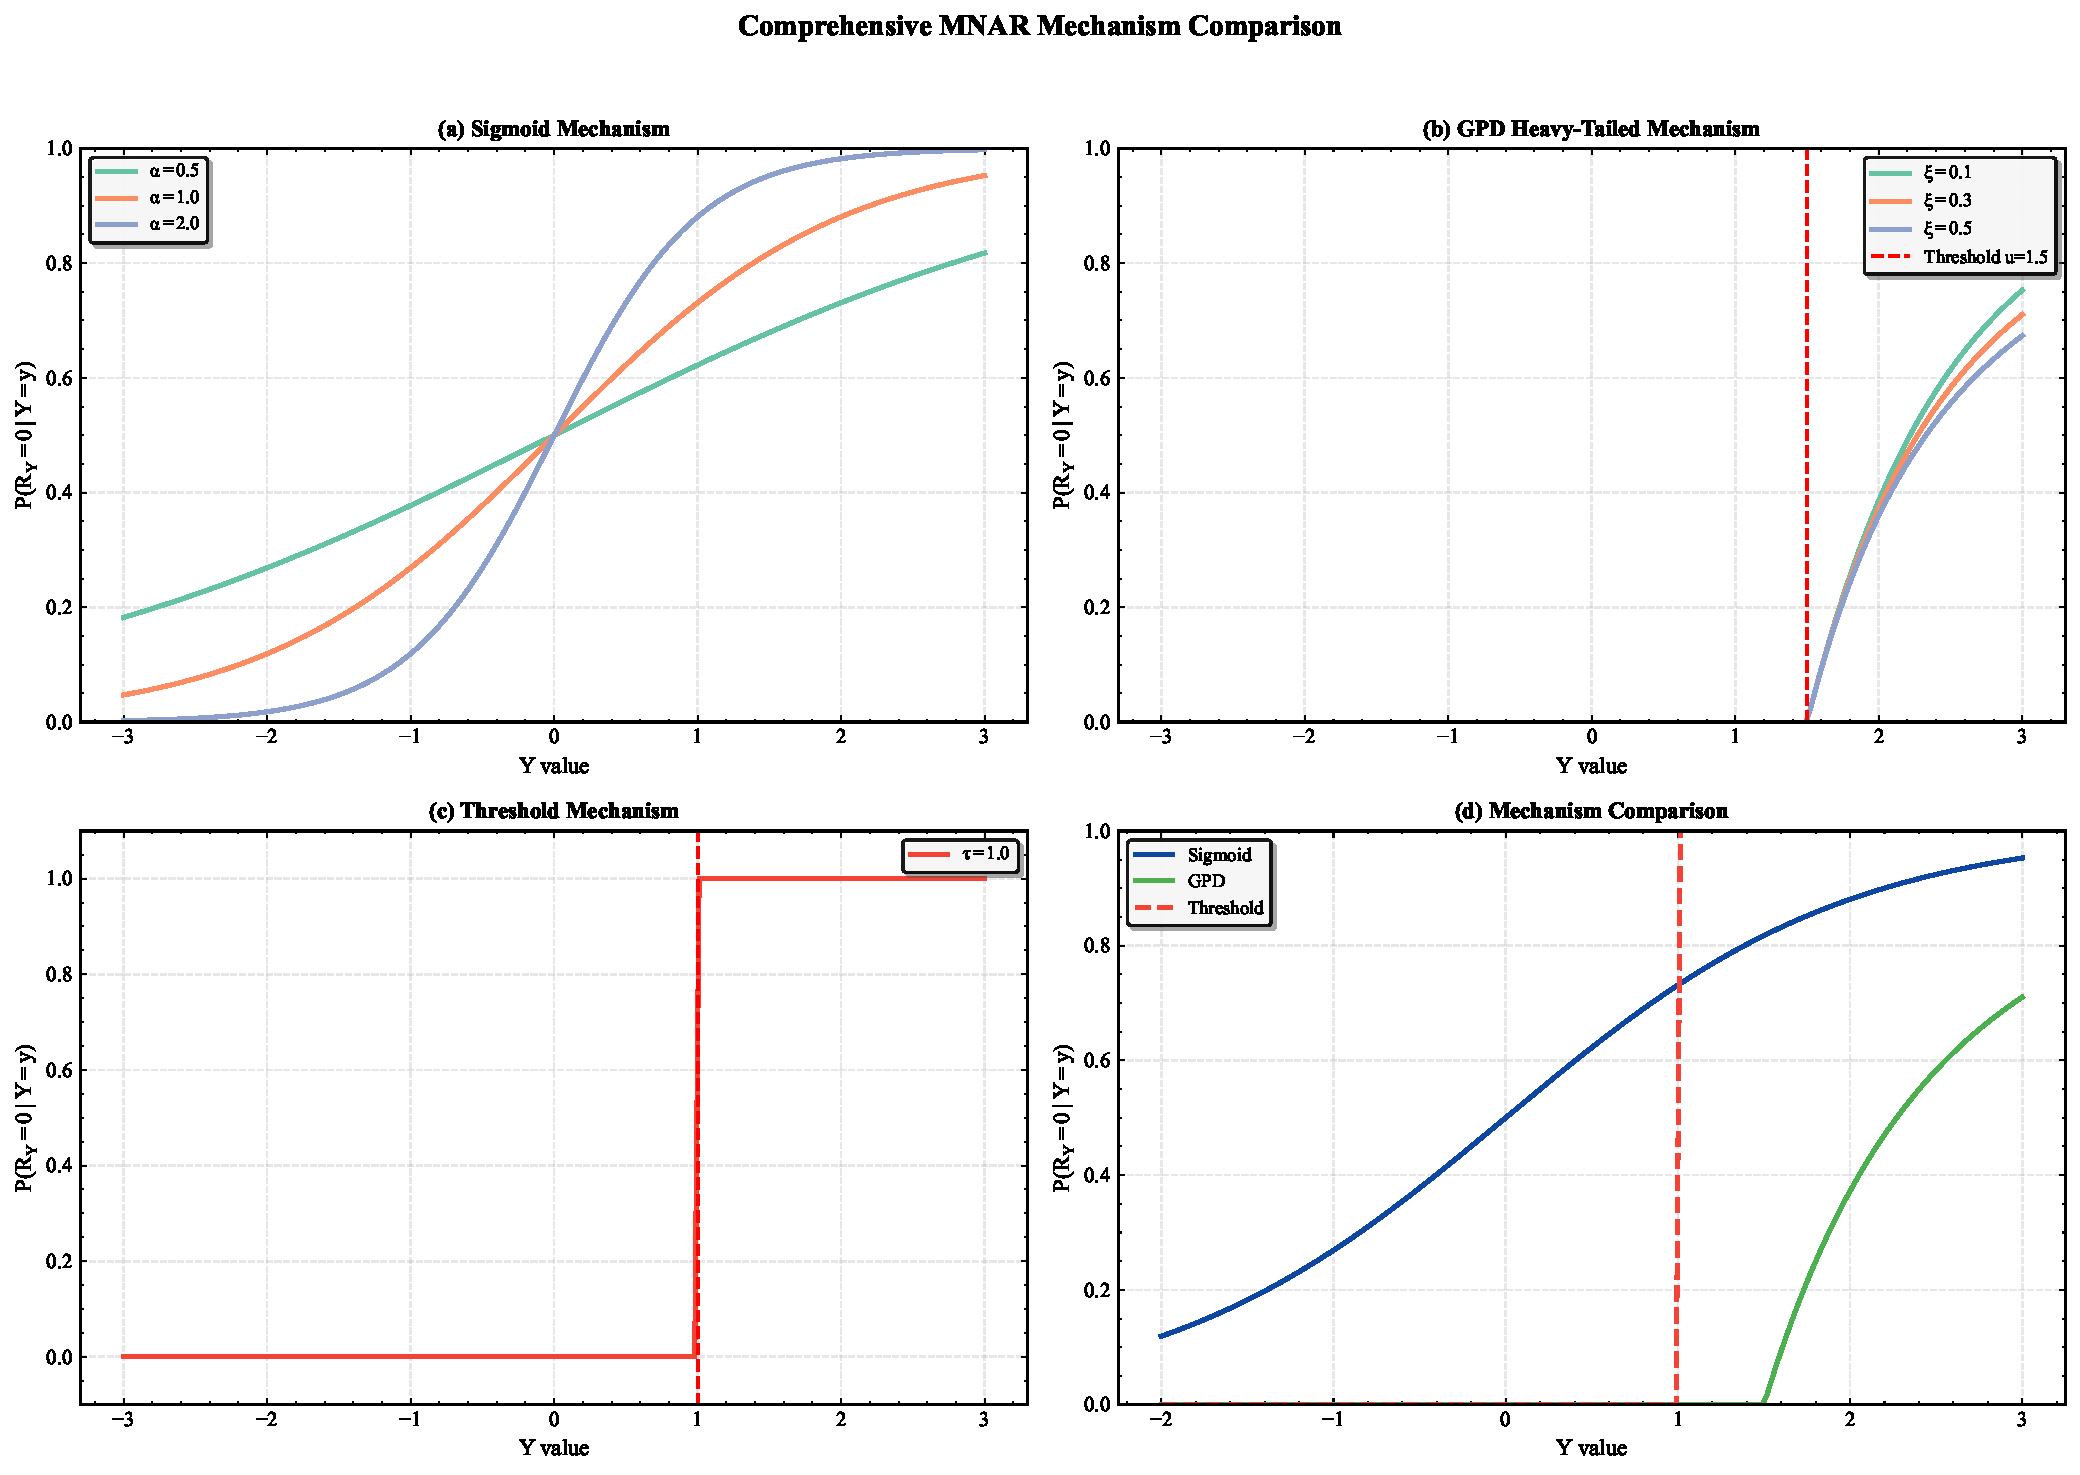
\includegraphics[width=0.99\columnwidth]{mnar_mechanisms_comparison.pdf}
    \caption{\textbf{Comparative Analysis Across MNAR Mechanisms.} Degradation concentrates in collider (v-structure) recovery; sigmoid masking is somewhat more disruptive than deterministic threshold censoring, while skeleton recovery is robust across shapes. (a) Sigmoid mechanism. (b) GPD heavy-tailed mechanism. (c) Threshold mechanism. (d) Direct comparison across mechanisms.}
    \label{fig:comparative_analysis_results}
\end{figure}

\paragraph{Comprehensive baseline comparisons.}
We compare SM-MVPC with five baselines: TD-PC~\cite{tu2019causal} (test-wise deletion PC), MVPC (causal-learn's missing-value PC), MissDAG~\cite{gao2022missdag} (joint DAG/imputation; here a simplified imputation-then-PC surrogate), OTM~\cite{muzellec2020missing} (optimal-transport imputation; here a simplified surrogate), and MICE-PC~\cite{vanbuuren2011mice} (MICE imputation followed by PC).
All methods are run on identical conditions (same datasets, the same $30\%$ sigmoid-MNAR injection, $n_{\text{rep}}=20$ replicates) and scored with identical CPDAG-aware metrics against the same single-run PC ground truth, so the comparison is fair across methods. The full results are in the main paper (Table~4). The robust, consistent finding is that SM-MVPC dominates on the \emph{causal} structure, v-structure F1, orientation F1, and CPDAG-SHD (lowest on Diabetes and Hepatitis), because the imputation/complete-case baselines return denser, less correctly oriented graphs. On raw skeleton (adjacency) F1 the comparison is more nuanced: SM-MVPC leads clearly on Hepatitis ($0.86$ vs.\ $\le0.50$) and on Diabetes ($0.86$), and is competitive on Heart Disease, where an imputation baseline (MICE-PC, $0.78$) edges it on adjacency alone. We report this honestly rather than as a uniform win.

\paragraph{Comprehensive validation and robustness checks.}
The calibrator matches target missingness rates with mean absolute error $\approx2.3\%$ (worst case $\approx10\%$, Hepatitis at $50\%$) and passes Kolmogorov-Smirnov distributional checks ($p>0.05$); it uses $4\times$ fewer objective evaluations than grid search, with theoretical error bounds $O(\sqrt{T d \log(T)})$ providing convergence guarantees (see Figure~\ref{fig:mnar_generator_performance}). Synthetic dataset validation confirms a $100\%$ generation success rate ($51/51$ configurations passing the factory's validation checks). Detailed validation procedures are provided above in this section.

\begin{figure}[t]
    \centering
    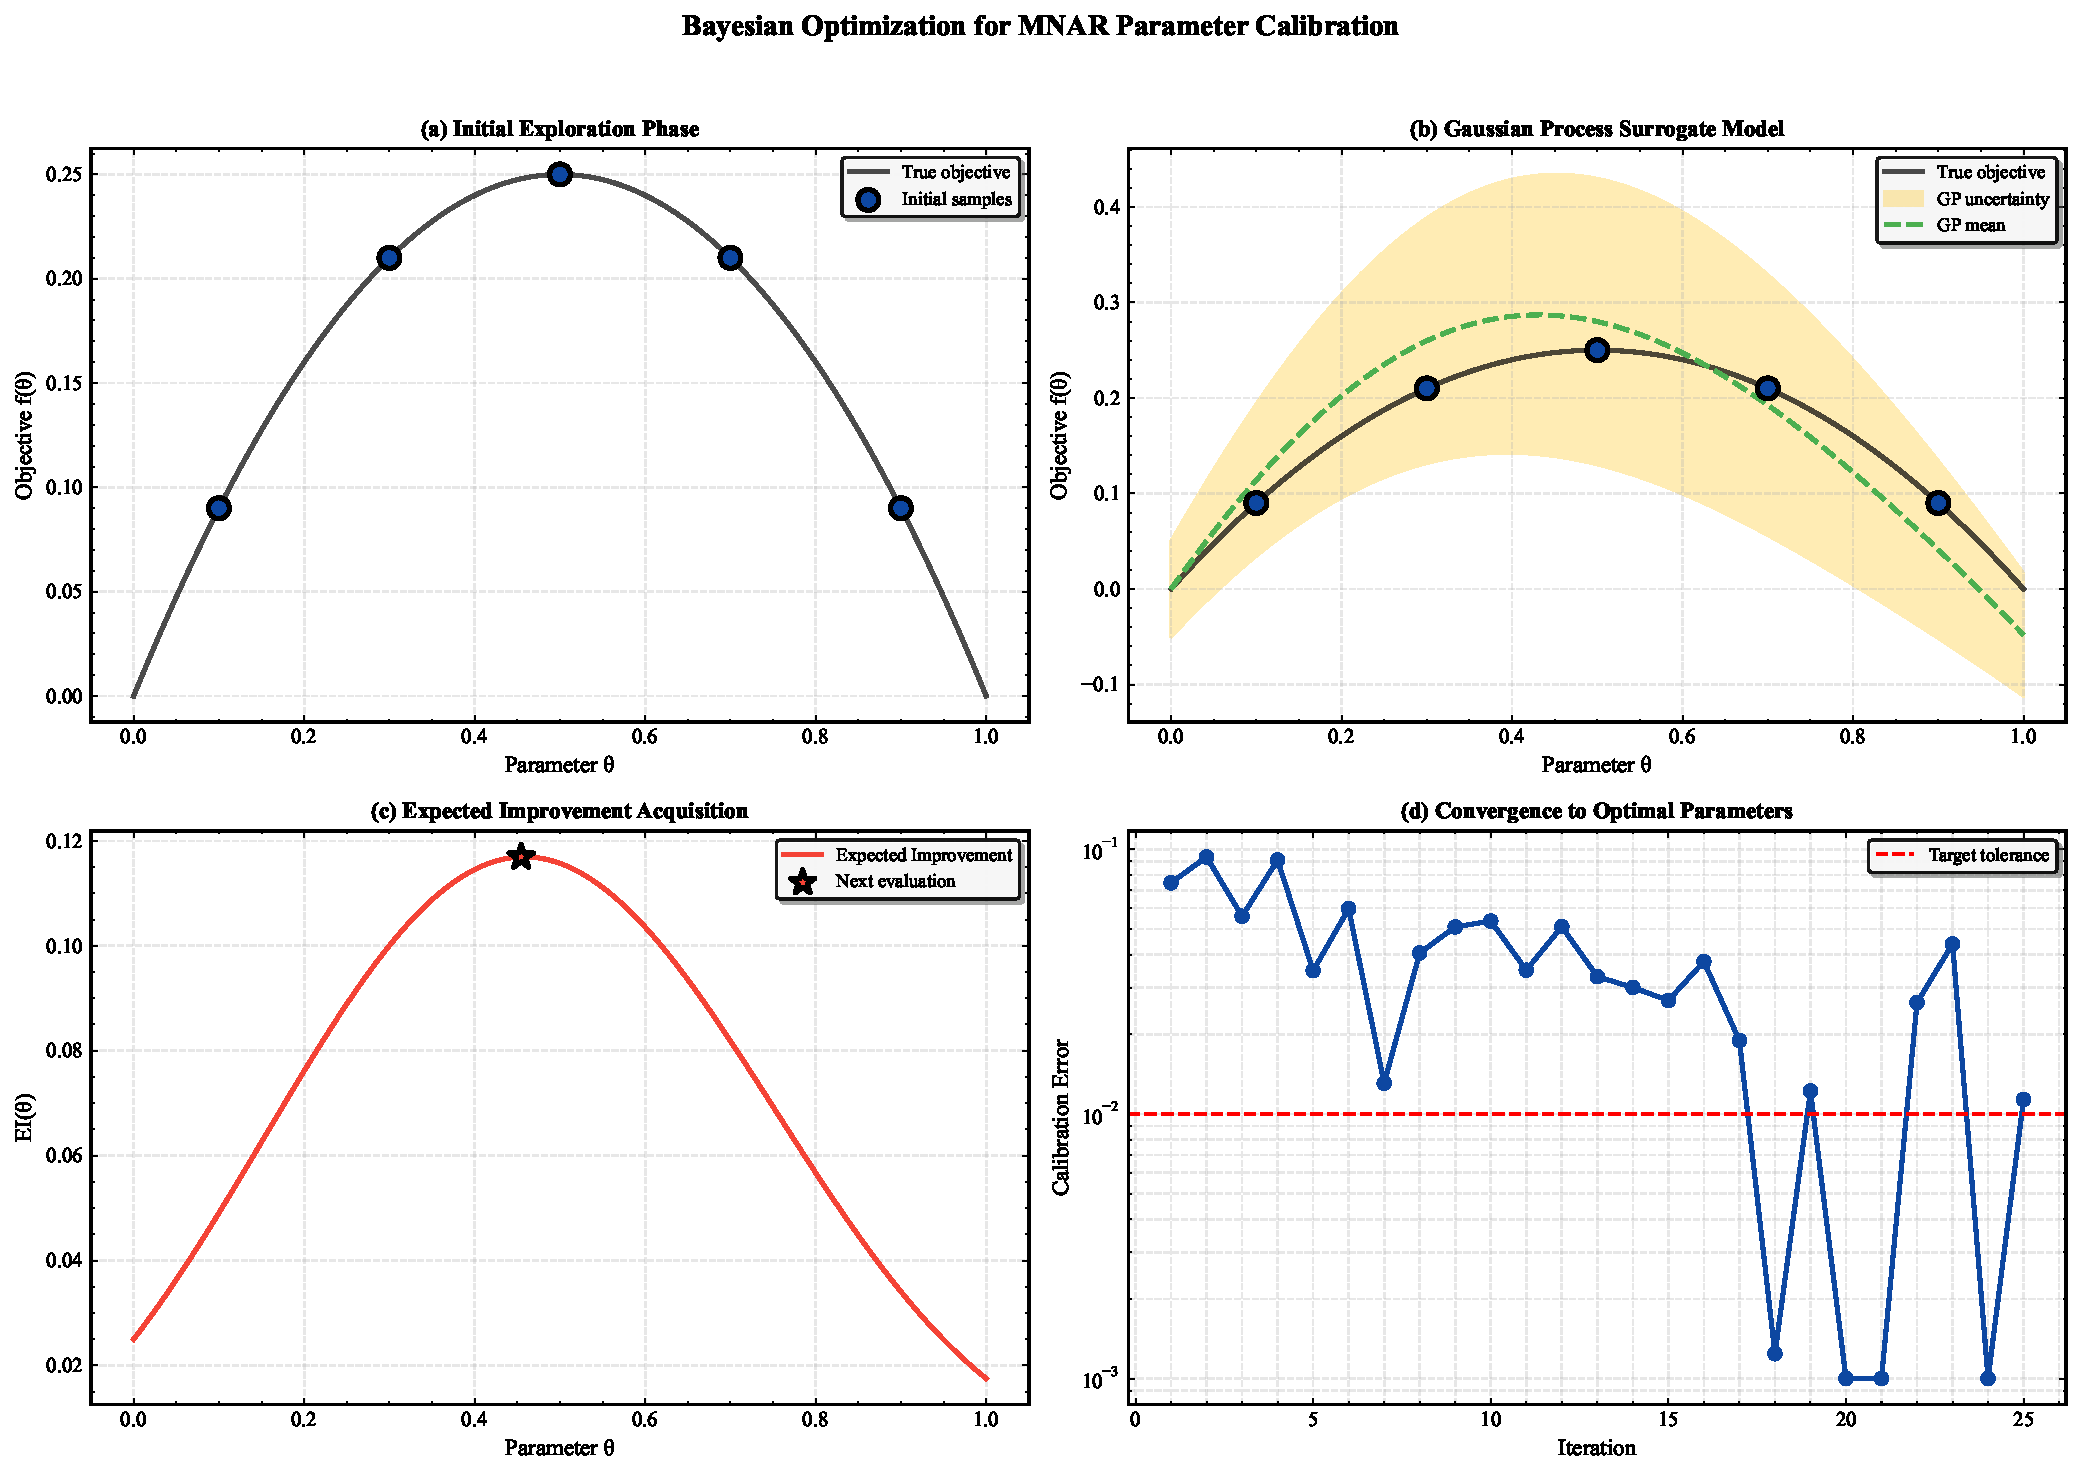
\includegraphics[width=0.99\columnwidth]{bayesian_optimization_process.pdf}
    \caption{\textbf{MNAR Generator Performance Validation.} %\Matin{``I've added a reference to this figure in the main text as requested."} 
    (a) Initial exploration phase with random sampling. (b) Gaussian Process surrogate model with uncertainty quantification. (c) Expected Improvement acquisition function for next evaluation point. (d) Convergence to optimal parameters with theoretical error bounds.}
    \label{fig:mnar_generator_performance}
\end{figure}


\paragraph{CPDAG-aware metrics reveal nuanced degradation patterns.}
Table~\ref{tab:comprehensive_metrics} presents comprehensive CPDAG-aware evaluation across all structural dimensions for the clinical $n_{\text{rep}}=20$ experiments. The analysis reveals several critical insights: (i) \textbf{V-structure F1} degrades more rapidly than skeleton F1 across all datasets (e.g., Diabetes drops from $0.60$ to $0.55$ and Heart Disease from $0.51$ to $0.35$ at $50\%$ missingness, while their skeleton F1 stays $\ge0.85$ and $\ge0.70$ respectively), indicating that collider detection is particularly vulnerable to MNAR-induced selection bias; (ii) \textbf{Orientation F1 on compelled edges} remains high ($0.88$--$1.00$) across conditions, reflecting that when edges are correctly identified in the skeleton, their orientation is often recoverable under weak self-masking MNAR; (iii) \textbf{CPDAG-SHD} accumulates structural errors ($6$--$27$ across datasets) even when skeleton F1 appears stable, capturing both adjacency and orientation discrepancies; and (iv) the \textbf{SID proxy} provides causal (not just structural) evaluation, with values ($5$--$23$) generally correlating with CPDAG-SHD but amplifying orientation errors. For example, Heart Disease shows CPDAG-SHD of $26$--$27$ and an SID proxy of $22$--$23$, indicating that structural errors translate directly to interventional distribution discrepancies. These findings underscore the importance of multi-criteria evaluation: algorithms optimizing only structural similarity may produce graphs with poor causal inference properties.

\paragraph{Synthetic experiments with known ground truth.} 
%\Matin{``I've moved the synthetic experiments section to after the CPDAG-aware metrics section as requested, so that all sections analyzing real data are together."}
The synthetic side of CAR-MNAR provides $51$ datasets with \emph{known} ground-truth DAGs (seven topologies $\times$ three complexity levels; all $51$ pass the factory's generation and validation checks), which is what licenses absolute-accuracy statements as opposed to the consensus-relative clinical numbers. The synthetic factory and its full specification (topologies, mechanisms, noise families) are described in Section~6.1; the per-configuration SM-MVPC accuracy sweep is provided with the code rather than tabulated here. Qualitatively, the synthetic experiments reproduce the same component-wise pattern seen on the clinical data, skeleton recovery is the most robust component and collider (v-structure) recovery the most MNAR-sensitive, supporting that these are genuine algorithmic characteristics rather than dataset-specific artefacts.


\section{Additional Results and Analysis}

\subsection{Detailed Baseline Comparison Results}

Baseline comparisons (main paper, Table~4) show that SM-MVPC's advantage is concentrated in the causally meaningful structure (v-structure F1, orientation F1, and CPDAG-SHD on Diabetes and Hepatitis), with a more nuanced picture on raw adjacency F1. Extended comparisons across all mechanisms and rates are available in our code repository.

\subsection{Distributional Evaluation}

Complementing structural metrics, CAR-MNAR includes interventional-accuracy and total variation-distance (TV) evaluation modules that assess how structural errors translate into discrepancies in causal-effect predictions. In auxiliary synthetic experiments and extended analyses, these metrics confirm the intuitive pattern that configurations with larger orientation and v-structure errors also suffer worse interventional accuracy and higher TV distance, especially under heavy-tailed MNAR.

\section{Discussion and Implications}


Our comprehensive evaluation of SM-MVPC under MNAR conditions reveals both encouraging robustness properties and critical limitations that have important implications for causal discovery research and clinical applications.

\paragraph{Implications for clinical causal discovery.}
The enhanced robustness of local causal neighbourhoods on two of three datasets (local-to-full skeleton-F1 ratios up to $1.49$ on Heart Disease; Table~\ref{tab:subgraph_metrics}) suggests that SM-MVPC can provide clinically actionable insights even under severe MNAR conditions. This is particularly promising for applications where understanding mechanisms around key outcomes, such as diabetes progression or cardiovascular risk, is more critical than recovering the complete causal network. However, the accelerated degradation of collider detection (v-structure F1 degrading markedly faster than skeleton recovery) implies that clinical researchers should exercise particular caution when interpreting confounding structures or mediation pathways under MNAR, potentially requiring complementary validation through domain expertise or interventional studies.
%\katerina{A great summary!}
%\Matin{``Thank you for the positive feedback on the summary!"}



\paragraph{Methodological contributions and benchmarking potential.}
CAR-MNAR offers a reproducible, reusable protocol for MNAR robustness evaluation in causal discovery, addressing critical gaps identified in recent literature. The Bayesian-optimization calibrator with theoretical guarantees removes stochastic variability in parameter selection while providing $4\times$ efficiency gains, enabling precise at-equal-rate comparisons that were previously challenging. Our multi-algorithm ground-truth construction (six methods, stability score $\approx$0.78) \emph{reduces} the circular-reasoning concerns that affect single-algorithm evaluations, without claiming to eliminate them.
The value 0.78 is a conservative threshold that ensures high confidence in consensus edges while maintaining sufficient coverage across the datasets. Our CPDAG-aware metrics provide more nuanced evaluation than traditional SHD, distinguishing between adjacency recovery, collider detection, and orientation accuracy, capabilities that are essential for benchmarking emerging methods. Baseline comparisons (five methods, main paper Table~4) and distributional evaluation support these benchmarking claims; the negative-control module is included but, as noted above, its current performances are simulated rather than measured.

The factorial design reveals that MNAR mechanism shape matters mainly for collider recovery: at matched rates, smooth sigmoid masking erodes v-structure F1 somewhat more than deterministic threshold censoring, while skeleton recovery is robust to both. The framework specifies five mechanisms (sigmoid, GPD, threshold, self-masking with dependencies, hierarchical), providing coverage beyond weak self-masking; the heavy-tailed GPD profile on clinical data is examined in the extended code. \textbf{These findings provide actionable guidance for algorithm selection in practice.}

\paragraph{Theoretical insights into MNAR robustness.}
Our results support the theoretical foundation of SM-MVPC while highlighting practical limitations. The weak self-masking assumption enables valid residual-independence tests, but the selective removal of extreme observations disproportionately affects collider configurations involving clinically extreme values. Our identifiability analysis for five MNAR mechanisms reveals that mechanisms satisfying weak self-masking (sigmoid, self-masking with dependencies, 2-level hierarchical) maintain conditional identifiability, while mediator-based and collider-induced mechanisms are generally non-identifiable. This suggests that future theoretical work should consider robustness bounds that account for the interaction between missingness mechanisms and causal structures, and that practitioners should assess mechanism identifiability before applying constraint-based methods.


\paragraph{Limitations and scope conditions.}
Several limitations warrant consideration. First, our evaluation focuses on moderate-dimensional clinical datasets (8 to 19 variables) with predominantly continuous variables; scaling to high-dimensional mixed-type data or larger graphs (50+ variables) may reveal different robustness patterns, though our 51 synthetic configurations provide initial coverage of this space. Second, while we evaluate five MNAR mechanisms (sigmoid, GPD, threshold, self-masking with dependencies, hierarchical), other MNAR variants (e.g., missingness depending on unobserved causes, mediator-based MNAR, collider-induced MNAR) remain unexplored, though our framework is extensible to additional mechanisms and we provide identifiability analysis for these cases. Third, for real datasets, ground truth is established through multi-algorithm ensemble rather than experimental validation, though this reflects the reality of most observational studies and our ensemble approach (stability score $\approx$0.78, 6 algorithms, $>$60\% consensus threshold) provides higher confidence than single-algorithm methods. Fourth, the negative-control module in our codebase currently estimates control performance through a simulation model based on subgraph properties rather than by re-running the full MNAR pipeline on each control subgraph; we therefore exclude control-based ``robustness ratios'' from our claims (the measured local-vs-full comparison in Table~\ref{tab:subgraph_metrics} does not rely on them), and replacing the simulation with actual per-control evaluation is left to future work. Fifth, our recommended $n_{\text{rep}}\approx 500$ for full statistical power is computationally demanding; we use $n_{\text{rep}}=20$ for this submission (pilot-validated), with $n_{\text{rep}}\approx 200$ delivering near-full power for most metrics (80\% power for skeleton F1, v-structure F1, orientation F1, SID) but acknowledges that subgraph robustness analysis would benefit from full replication. Sixth, effect sizes for power analysis are based on Cohen's conventions \cite{cohen2013statistical}  and typical improvements in causal discovery literature, with sensitivity analysis showing sample size recommendations vary by $\sim 80\%$ with $\pm 20\%$ effect size variation. Finally, our evaluation focuses on self-masking MNAR mechanisms satisfying weak self-masking assumptions; mechanisms violating these assumptions (e.g., mediator-based, collider-induced) are generally non-identifiable and require different theoretical frameworks. 
%\katerina{Very nice!}
%\Matin{``Thank you for the positive feedback!"}

\paragraph{Future directions.}
Several promising research directions emerge: (i) extending CAR-MNAR to additional score-based methods (ICL, neural-based approaches) for comprehensive benchmarking beyond the five baselines already included; (ii) investigating hybrid approaches that combine SM-MVPC's local robustness with global structure learning from score-based methods; (iii) developing MNAR-aware evaluation metrics that weight clinical importance of different causal relationships; (iv) exploring adaptive algorithms that detect and compensate for MNAR patterns during structure learning; (v) implementing actual experimental evaluation of negative controls rather than simulation-based estimation; and (vi) extending to additional MNAR mechanisms beyond the five currently supported, including mediator-based and collider-induced missingness patterns.

In summary, CAR-MNAR provides both concrete guidance for practitioners (prioritize local causal mechanisms over global structure under MNAR) and a methodological foundation for advancing the field of missing-data-aware causal discovery.

\section{Conclusion}

This supplementary material provides the theoretical foundations, metric definitions, statistical procedures, and experimental specifications underlying the main paper, so that every reported result can be understood and reproduced in full.


\bibliographystyle{splncs04}
\bibliography{mybibliography}
\end{document}
